\documentclass{article}
\AtBeginDocument{\RenewCommandCopy\qty\SI}
\usepackage{style}
\title{ECE358 Cheatsheet}
\author{Hanhee Lee}
\lhead{ECE358}
\rhead{Hanhee Lee}

\begin{document}
\maketitle

\tableofcontents

\listoffigures

\listoftables

Read the textbook for this course.

% W1
\section{Asymptotics (Ch. 3.1-2 pg. 50-63, L2)} %DONE except for 2nd page of L2.
Asymptotic efficiency focuses on understanding how the running time of an algorithm grows with the input size, particularly for large inputs.
\subsection{Big-O (Upper Bound)}
    \begin{definition} 
        $ f(n) = O(g(n)) \text{ iff } \exists \text{ positive constants } c \text{ and } n_0 \text{ s.t. } 0 \leq f(n) \leq c g(n) \; \forall \; n \geq n_0 $
        \begin{itemize}
            \item \textbf{Asymptotic upper bound:} Grows \textbf{no faster} than a certain rate, based on the highest-order term.
        \end{itemize}
    \end{definition}

    \begin{warning}
        Every function $f(n)$ in the set $O(g(n))$ must be \textbf{asymptotically nonnegative} (i.e. $f(n)$ must be positive whenever $n$ is sufficiently large).
    \end{warning}

    \begin{example}
        To show that \( 13n + 7 \in O(n) \), we need to find constants \( c > 0 \) and \( n_0 > 0 \) such that:

        \[
        13n + 7 \leq c \cdot n \quad \text{for all } n \geq n_0.
        \]

        \begin{enumerate}
            \item Start with the inequality:
            
            \[
            13n + 7 \leq c \cdot n.
            \]
            
            \item Rearrange the inequality to isolate \( c \):
            
            \[
            13n + 7 \leq c \cdot n \implies 13 + \frac{7}{n} \leq c.
            \]
            
            \item For this inequality to hold for all \( n \geq n_0 \), choose \( n_0 \) such that \( \frac{7}{n_0} \) is sufficiently small.
            
            \item Set \( n_0 = 7 \):
            
            \[
            \frac{7}{n_0} = \frac{7}{7} = 1.
            \]
            
            Now the inequality becomes:
            
            \[
            13 + \frac{7}{7} = 13 + 1 = 14 \leq c.
            \]
            
            \item Choose \( c = 14 \). This choice satisfies:
            
            \[
            13 + \frac{7}{n} \leq 14 \quad \text{for all } n \geq 7.
            \]
            
            \item Therefore, with \( c = 14 \) and \( n_0 = 7 \), we have:
            
            \[
            13n + 7 \leq 14n \quad \text{for all } n \geq 7.
            \]
        \end{enumerate}
    \end{example}

    \begin{example}
        To prove that \( \frac{1}{2}n^2 - 3n \in O(n^2) \), we need to show:

        \[
        \frac{1}{2}n^2 - 3n \leq C \cdot n^2 \quad \text{for some constants } C > 0 \text{ and } n_0 > 0 \text{, for all } n \geq n_0.
        \]

        \begin{enumerate}
            \item Start with the inequality we want to prove:
            
            \[
            \frac{1}{2}n^2 - 3n \leq C \cdot n^2.
            \]
            
            \item Rearrange the inequality to isolate \( C \):
            
            \[
            \frac{1}{2}n^2 - 3n \leq C \cdot n^2 \implies \frac{1}{2} - \frac{3}{n} \leq C.
            \]
            
            \item For the inequality to hold for all \( n \geq n_0 \), we need to make \( \frac{3}{n} \) sufficiently small:
            
            \item Set \( n_0 = 1 \). For \( n \geq 1 \):
            
            \[
            \frac{3}{n} \leq 3 \quad \Rightarrow \quad \frac{1}{2} - \frac{3}{n} \leq \frac{1}{2} - 3.
            \]
            
            However, this inequality might lead to negative values for smaller \( n \), so we adjust \( C \) accordingly.
            
            \item Choose \( C = \frac{7}{2} \). With this choice:
            
            \[
            \frac{1}{2} - \frac{3}{n} \leq C \quad \text{for all } n \geq 1.
            \]
            
            Setting \( C = 3.5 \) ensures that:
            
            \[
            \frac{1}{2} - \frac{3}{n} \leq 3.5 \quad \text{holds for all } n \geq 1.
            \]
            
            \item Therefore, with \( C = 3.5 \) and \( n_0 = 1 \), we have:
            
            \[
            \frac{1}{2}n^2 - 3n \leq 3.5n^2 \quad \text{for all } n \geq 1.
            \]
        \end{enumerate}

        This confirms that \( \frac{1}{2}n^2 - 3n \in O(n^2) \).
    \end{example}

    \begin{warning}
        The choice of $C=3.5$ was just one option. Any constant C that satisfies the inequality works. It doesn't have to be the tightest bound for big-O.
    \end{warning}

    \begin{example}
        \[
        n! = 1 \cdot 2 \cdot 3 \cdot 4 \cdot \ldots \cdot n \leq n \cdot n \cdot n \cdot \ldots \cdot n = O(n^n) \quad \text{(with \( n \) terms)}
        \]

        Similarly:

        \[
        \log n! = O(n \log n) = O(\log n^n)
        \]
    \end{example}

    \begin{example}
        \textbf{Statement:} Prove that $2^{n+1} = O(2^n)$.
        
        \textbf{Step 1:} Begin by noting that $2^{n+1}$ can be rewritten as:
        \[
        2^{n+1} = 2 \cdot 2^n
        \]
        We want to show that $2^{n+1} \leq C \cdot 2^n$ for some constant $C$ and for all $n \geq n_0$.
        
        \textbf{Step 2:} To satisfy the definition of Big-O, we need:
        \[
        0 \leq 2 \cdot 2^n \leq C \cdot 2^n \quad \forall n \geq 0
        \]
        This inequality holds if $C \geq 2$, as the factor of 2 on the left-hand side is less than or equal to $C$.
        
        \textbf{Step 3:} Let us choose $C = 3$ and $n_0 = 1$. Now check the inequality for all $n \geq n_0$:
        \[
        0 \leq 2 \cdot 2^n \leq C \cdot 2^n \quad \forall n \geq n_0
        \]
        This is true because $2 \cdot 2^n \leq 3 \cdot 2^n$ holds for all $n \geq 1$.
        
        \textbf{Conclusion:} Therefore, we have shown that:
        \[
        2^{n+1} = O(2^n)
        \]
    \end{example}
        

    \begin{example}
        \textbf{Statement:} Prove that $2^{n+1} = \Omega(2^n)$.
        
        \textbf{Step 1:} Recall the definition of $\Omega$: we need to show that $2^{n+1} \geq C \cdot 2^n$ for some constant $C > 0$ and for all $n \geq n_0$.
        
        \textbf{Step 2:} Again, we can rewrite $2^{n+1}$ as:
        \[
        2^{n+1} = 2 \cdot 2^n
        \]
        We want to show:
        \[
        0 \leq C \cdot 2^n \leq 2 \cdot 2^n \quad \forall n \geq 0
        \]
        This inequality holds if $C \leq 2$.
        
        \textbf{Step 3:} Let us choose $C = 1$ and $n_0 = 1$. Now verify the inequality:
        \[
        0 \leq C \cdot 2^n \leq 2 \cdot 2^n \quad \forall n \geq 1
        \]
        This is true because $1 \cdot 2^n \leq 2 \cdot 2^n$ holds for all $n \geq 1$.
        
        \textbf{Conclusion:} Therefore, we have shown that:
        \[
        2^{n+1} = \Omega(2^n)
        \]
    \end{example}

\subsection{Big-Omega (Lower Bound)}
    \begin{definition}
        $ f(n) = \Omega(g(n)) \text{ iff } \exists \text{ positive constants } c \text{ and } n_0 \text{ such that } 0 \leq c g(n) \leq f(n) \; \forall \; n \geq n_0 $
        \begin{itemize}
            \item \textbf{Asymptotic lower bound:} Grows \textbf{at least as fast} as a certain rate, based on the highest-order term.
        \end{itemize}
    \end{definition}

    \begin{example}
        \begin{enumerate}
            \item The sum can be approximated by considering that the sequence is bounded above by:
        
            \[
            1 + 2 + 3 + \ldots + n \geq \left\lceil \frac{n}{2} \right\rceil + \left( \left\lceil \frac{n}{2} \right\rceil + 1 \right) + \ldots + n.
            \]
        
            \item Grouping terms to form pairs around the middle:
        
            \[
                \left\lceil \frac{n}{2} \right\rceil + \left( \left\lceil \frac{n}{2} \right\rceil + 1 \right) + \ldots + n \geq \left\lceil \frac{n}{2} \right\rceil \times \left\lceil \frac{n}{2} \right\rceil = \left\lceil \frac{n^2}{4} \right\rceil
            \]
        
            \item To express this in terms of \( \Omega(n^2) \), note that:
        
            \[
            \left\lceil \frac{n^2}{4} \right\rceil \geq \frac{n^2}{4}
            \]
        
            \item This implies:
        
            \[
            \left( \frac{1}{n} \right)n^2 = \Omega(n^2)
            \]
        
            \item Finding \( n_1 \): We choose \( n_1 \) such that the inequality holds for all \( n \geq n_1 \). Let's find \( n_1 \) by ensuring:
        
            \[
            \left\lceil \frac{n^2}{4} \right\rceil \geq c \cdot n^2
            \]
        
            Choosing \( c = \frac{1}{4} \), we need \( \left\lceil \frac{n^2}{4} \right\rceil \geq \frac{n^2}{4} \). This inequality naturally holds for \( n \geq 1 \). Thus, we can choose \( n_1 = 1 \), which gives:
        
            \[
            \left\lceil \frac{n^2}{4} \right\rceil = \Omega(n^2)
            \]
        
            This satisfies the inequality for all \( n_1 \geq 1 \).
        \end{enumerate}
        
        Thus, the sum \( 1 + 2 + 3 + \ldots + n \) is \( \Omega(n^2) \), indicating a quadratic lower bound.        
    \end{example}

\subsection{Big-Theta (Tight Bound)}
    \begin{definition}
        $ f(n) = \Theta(g(n)) \text{ iff } \exists \text{ positive constants } c_1, \; c_2, \; n_0 \text{ s.t. } 0 \leq c_1 g(n) \leq f(n) \leq c_2 g(n) \; \forall \; n \geq n_0 $
        \begin{itemize}
            \item \textbf{Asymptotically tight bounds:} Grows \textbf{precisely} at a certain rate, based on the highest-order term.
        \end{itemize}
    \end{definition}

    \begin{example}
        Consider the sum \( 1 + 2 + 3 + \ldots + n \), prove that it is $\Theta(n^2)$
        \begin{enumerate}
            \item From the previous example with Big-Omega, we know that $\Omega(n^2)$
            \item The sum can be written as:

            \[
            1 + 2 + 3 + \ldots + n = \frac{n(n+1)}{2}
            \]
        
            \item Expanding the expression:
        
            \[
            = \frac{1}{2}n^2 + \frac{1}{2}n
            \]
        
            \item Therefore, this sum is:
        
            \[
            = O(n^2)
            \]
            \item By Theorem 3.1, $\Theta(n^2)$.
        \end{enumerate}
    \end{example}

    \begin{example}
        Let \( f(n) = \sum_{i=1}^n i^k \). We want to show that \( f(n) = \Omega(n^{k+1}) \) and \( f(n) = O(n^{k+1}) \), indicating that \( f(n) \) is asymptotically bounded both above and below by \( n^{k+1} \).

        \begin{enumerate}

            \item Prove that \( f(n) = O(n^{k+1}) \):
            
            \begin{enumerate}
                \item Start with the definition of \( f(n) \):
                
                \[
                f(n) = \sum_{i=1}^n i^k.
                \]
                
                \item Observe that each \( i^k \) is less than or equal to \( n^k \) for \( i \leq n \). Therefore, we can bound the sum from above:
                
                \[
                \sum_{i=1}^n i^k \leq \sum_{i=1}^n n^k = n^k + n^k + \ldots + n^k = n \cdot n^k = n^{k+1}.
                \]
                
                \item This implies:
                
                \[
                f(n) = O(n^{k+1}),
                \]
                
                where the constant \( C \) can be chosen as 1. Thus, there exists a constant \( C > 0 \) such that \( f(n) \leq C \cdot n^{k+1} \) for sufficiently large \( n \).
                
            \end{enumerate}

            \item Prove that \( f(n) = \Omega(n^{k+1}) \):
            
            \begin{enumerate}
                \item To establish a lower bound, consider using a double sequence method:
                
                \[
                2f(n) = \sum_{i=1}^n i^k + \sum_{i=1}^n (n-i+1)^k.
                \]
                
                \item Notice that the first sum is ascending (i.e., \( 1^k + 2^k + \ldots + n^k \)) and the second sum is descending (i.e., \( n^k + (n-1)^k + \ldots + 1^k \)):
                
                \[
                2f(n) = \sum_{i=1}^n i^k + \sum_{i=1}^n (n-i+1)^k.
                \]
                
                \item Each pair \( i^k + (n-i+1)^k \) is greater than or equal to \( \left(\frac{n}{2}\right)^k \):
                
                \[
                2f(n) \geq \sum_{i=1}^n \left(\frac{n}{2}\right)^k = \left(\frac{n}{2}\right)^k + \ldots + \left(\frac{n}{2}\right)^k = n \cdot \left(\frac{n}{2}\right)^k = \frac{n^{k+1}}{2^k}.
                \]
                
                \item This simplifies to:
                
                \[
                2f(n) \geq \frac{n^{k+1}}{2^k} \Rightarrow f(n) \geq \frac{n^{k+1}}{2^{k+1}}.
                \]
                
                \item Therefore:
                
                \[
                f(n) = \Omega(n^{k+1}),
                \]
                
                showing that \( f(n) \) has a quadratic lower bound.
                
            \end{enumerate}

        \end{enumerate}

        \textbf{Conclusion:} Since \( f(n) \) is bounded above and below by \( n^{k+1} \), we conclude:

        \[
        f(n) = \Theta(n^{k+1}).
        \]
    \end{example}

    \begin{example}
        Show that $(n + a)^b = \Theta(n^b)$
        \begin{enumerate}
            \item \textbf{Key Observation:}
                \[
                n + a \leq n + |a| \leq 2n \quad \text{if} \ n \geq |a|
                \]
                \[
                n + a \geq n - |a| \geq \frac{1}{2} n \quad \text{if} \ n \geq 2|a|
                \]
            
            \item $(n + a)^b = O(n^b):$
            \[
            0 \leq (n + a)^b \leq C \cdot n^b
            \]
            Let $n_0 = |a| \Rightarrow 0 \leq (n + a)^b \leq (2n)^b = 2^b n^b$.
            Therefore, let $C \geq 2^b$ and the above holds (i.e. using the key observation):
            \[
            \therefore (n + a)^b = O(n^b)
            \]

            \item $(n + a)^b = \Omega(n^b):$
            \[
            0 \leq C \cdot n^b \leq (n + a)^b
            \]
            Let $n_0 = 2|a| \Rightarrow (n + a)^b \geq \left(\frac{1}{2} n \right)^b = \left(\frac{1}{2} \right)^b n^b$.
            Therefore, let $0 < C \leq \left(\frac{1}{2}\right)^b$ and the above holds:
            \[
            \therefore (n + a)^b = \Omega(n^b)
            \]

            \item Conclusion:
            \[
            \therefore (n + a)^b = O(n^b) \quad \text{and} \quad (n + a)^b = \Omega(n^b) \Rightarrow (n + a)^b = \Theta(n^b)
            \]
            \end{enumerate}
    \end{example}

\customFigure[1]{00_Images/BigO_Omega_Theta_Notation.png}{Graphical examples of the Big-O, Big-Omega, and Big-Theta.}

\begin{intuition}
    In all asymptotic notations, you are trying to describe a function after $n_0$ (i.e. ignore all flunctuation before).
\end{intuition}

\subsection{Theorem 3.1}
    \begin{theorem}
        $f(n) = \Theta(g(n))$ iff $f(n) = O(g(n))$ and $f(n)=\Omega(g(n))$.
    \end{theorem}

\subsection{Small-O (Strictly Slower)}
\begin{definition}
    $f(n) = o(g(n)) \text{ iff } \forall c > 0, \exists n_0 > 0 \text{ s.t. } 0 \leq f(n) < c g(n) \text{ for all } n \geq n_0.$
\end{definition}

\subsection{Small-Omega (Strictly Faster)}
\begin{definition}
    $f(n) = \omega(g(n)) \text{ iff } \forall c > 0, \exists n_0 > 0 \text{ s.t. } 0 \leq c g(n) < f(n) \text{ for all } n \geq n_0.$
\end{definition}

\subsection{Asymptotic notation and running times}
    \begin{warning}
        Make sure that the asymptotic notation you use is as precise as possible without overstating which running time (i.e. worst-case, best-case, or any average/expected-case) it applies to.
    \end{warning}

\subsection{Abuses of asymptotic notation}
    \begin{intuition}
        \begin{itemize}
            \item \textbf{Equality:}
            \begin{itemize}
                \item When asymptotic notation stands alone on the RS of an equation (or inequality), then $= \text{ means } \in$.
                \item When asymptotic notation is in a formula, it is an anonymous function (AF) that we do not care to name.
                \item When asymptotic notation appears on the LS of an equation: No matter how the AF is chosen on the LS, there is a way to choose the AF on the RS to make the equation valid.
            \end{itemize}
            \item \textbf{Variable tending toward $\infty$ must be inferred from context:}
            \begin{itemize}
                \item e.g. $O(g(n))$, then we are interested in the growth of $g(n)$ as $n$ grows.
                \item e.g. $f(n) = O(1)$, then $f(n)$ is bounded from above by a constant as $n$ goes to $\infty$.
                \item e.g. $T(n) = O(1) \text{ for } n<3$ is that there exists a positive constant $c$ such that $T(n) \leq c \text{ for } n<3$.
            \end{itemize}
        \end{itemize}
    \end{intuition}

\subsection{Comparing function properties}
    \begin{definition}
        
        \textbf{Transitivity:}
        \begin{itemize}
            \item $f(n) = \Theta(g(n)) \text{ and } g(n)=\Theta(h(n)) \text{ imply } f(n) = \Theta(h(n))$
            \item $f(n) = O(g(n)) \text{ and } g(n)=O(h(n)) \text{ imply } f(n) = O(h(n))$
            \item $f(n) = \Omega(g(n)) \text{ and } g(n)=\Omega(h(n)) \text{ imply } f(n) = \Omega(h(n))$
        \end{itemize}
        \vspace{1em}

        \textbf{Symmetry:}
        \begin{itemize}
            \item $f(n) = \Theta(g(n)) \text{ iff } g(n) = \Theta(f(n))$.
        \end{itemize}
        \vspace{1em}

        \textbf{Transpose symmetry:}
        \begin{itemize}
            \item $f(n) = O(g(n)) \text{ iff } g(n) = \Omega(f(n))$
        \end{itemize}
        \vspace{1em}

        \textbf{Different functions:}
        \begin{itemize}
            \item \( n^a = O(n^b) \), iff \( a \leq b \).
            \item \( \log_a(n) = O(\log_b(n)) \), $\forall$ \( a, b \).
            \item \( c^n = O(d^n) \), iff \( c \leq d \).
            \item If \( f(n) = O(f'(n)) \) and \( g(n) = O(g'(n)) \), then:
            \begin{enumerate}
                \item \( f(n) \cdot g(n) = O(f'(n) \cdot g'(n)) \).
                \item \( f(n) + g(n) = O(\max\{f'(n), g'(n)\}) \).
                \begin{itemize}
                    \item ' is not a derivative, just another function. 
                \end{itemize}
            \end{enumerate}
        \end{itemize}
        
    \end{definition}

    \begin{intuition}
        \begin{itemize}
            \item \( 1 \ll \log^*(n) \ll \log^i n \ll (\lg n)^a \ll n^b \ll c^n \quad \forall i, a, b, c \)
            
            \item \( f(n) \ll g(n) \Rightarrow h(n)f(n) \ll h(n)g(n) \)
            
            \item \( f(n) \ll g(n) \Rightarrow f(n)^{h(n)} \ll g(n)^{h(n)} \)
            
            \item \( f(n) \ll g(n) \) and \( \lim_{n \to \infty} h(n) > 1 \Rightarrow h(n)^{f(n)} \ll h(n)^{g(n)} \)
            
            \item Assume \( f \) and \( h \) are eventually positive, i.e. \( \lim_{n \to \infty} f(n) > 0 \) and \( \lim_{n \to \infty} h(n) > 0 \). 
            \begin{itemize}
                \item Note: \( f(n) \ll g(n) \Rightarrow \lim_{n \to \infty} g(n) = \infty \)
            \end{itemize}
            
            \item \( f(n) \ll g(n) \) means \( f(n) = o(g(n)) \)
            
            \item Notice the direction of the replication.
        \end{itemize}    
    \end{intuition}

    \begin{derivation}
        In tutorial 2.
    \end{derivation}
    
        \subsubsection{Common justification steps}
        \begin{intuition}
            \begin{itemize}
                \item Exponential functions grow faster than polynomial functions, which grow faster than polylogarithmic functions.
                \item The base of a logarithm doesn’t matter asymptotically, but the base of an exponential and the degree of a polynomial do matter.
            \end{itemize}
        \end{intuition}

\subsection{Limit method}
    \begin{definition}
        Find the asymptotic relationship between two functions for which you might not have any intuition about. 
        \begin{equation}
            \lim_{n \to \infty} \frac{f(n)}{g(n)} = 0 \Rightarrow f(n) = o(g(n))
        \end{equation}
        
        \begin{equation}
            \lim_{n \to \infty} \frac{f(n)}{g(n)} = \infty \Rightarrow f(n) = \omega(g(n))
        \end{equation}
        
        \begin{equation}
            \lim_{n \to \infty} \frac{f(n)}{g(n)} < \infty \text{ i.e. is anything finite } \Leftrightarrow f(n) = O(g(n))
        \end{equation}
        
        \begin{equation}
            \lim_{n \to \infty} \frac{f(n)}{g(n)} > 0 \text{ i.e. non-zero } \Leftrightarrow f(n) = \Omega(g(n))
        \end{equation}
        
        \begin{equation}
            \lim_{n \to \infty} \frac{f(n)}{g(n)} = C \text{ s.t. } 0 < C < \infty \Leftrightarrow f(n) = \Theta(g(n))
        \end{equation}        
    \end{definition}

    \subsubsection{L'Hôpital's rule}
    \begin{definition}
        $\text{if } \lim_{x \to a} \frac{f(x)}{g(x)} = \frac{0}{0} \text{ or } \frac{\infty}{\infty}$ then,
        \begin{equation}
            \lim_{x \to c} \frac{f(x)}{g(x)} = \lim_{x \to c} \frac{f'(x)}{g'(x)}
        \end{equation}
        
    \end{definition}

    \begin{warning}
        $f(n)$ and $g(n)$ need to be different functions. 
    \end{warning}

\subsection{Polynomially-bounded}
\begin{definition}
    \begin{itemize}
        \item \textbf{Polylogarithmically bounded:} \( f(n) = O((\lg n)^k) \quad \exists k > 0 \)
        
        \item \textbf{Polynomially bounded:} \( f(n) = O(n^k) \quad \exists k > 0 \)
        
        \item \textbf{Exponentially bounded:} \( f(n) = O(k^n) \quad \exists k > 0 \)
    \end{itemize}
\end{definition}

\begin{intuition}
    \begin{itemize}
        \item \textbf{Notation:} \( (\lg n)^2 = (\lg n) \cdot (\lg n) \) (polylogarithmic) and \( \lg^2 n = \lg(\lg n) \) (iterated log). 
    \end{itemize}
\end{intuition}

\begin{theorem}
    $f(n) = O(n^k) \Leftrightarrow \lg(f(n)) = O(\lg n)$
\end{theorem}

\begin{theorem}
    All logarithmically bounded functions are polynomially bounded, i.e. \((\lg n)^a = O(n^b) \quad \forall a, b > 0\)
\end{theorem}

\begin{theorem}
    All polynomially bounded functions are exponentially bounded, i.e. \( f(n) = O(n^a) \Rightarrow f(n) = O(b^n) \quad \forall a > 0 \text{ and } \forall b > 1\)
\end{theorem}

\begin{derivation}
    In tutorial 2.
\end{derivation}

\subsection{Logarithm method}
    \begin{definition}
        \textbf{Limit of Logs:} $\lim_{x \to a} (\log_b f(x)) = \log_b \left( \lim_{x \to a} f(x) \right)$

        $\text{Suppose we want to compute } \lim_{n \to \infty} \frac{f(n)}{g(n)} = L$

        \[
        \therefore \lg \left( \lim_{n \to \infty} \frac{f(n)}{g(n)} \right) = \lg L
        \]

        \[
        \therefore \lim_{n \to \infty} \left( \lg \frac{f(n)}{g(n)} \right) = \lg L
        \]

        \[
        \therefore \lim_{n \to \infty} \frac{f(n)}{g(n)} = L = 2^{\lim_{n \to \infty} \lg \left( \frac{f(n)}{g(n)} \right)}
        \]
    \end{definition}

    \begin{example}
        \begin{enumerate}

            \item \textbf{Apply logarithm to the limit.}
            Start by taking the logarithm of the limit:
            \[
            \lg \left( \lim_{n \to \infty} \frac{2^{n+1}}{4^n} \right)
            \]
        
            \item \textbf{Move the logarithm inside the limit.}
            Since the logarithm function is continuous, we can move it inside the limit:
            \[
            \lim_{n \to \infty} \left( \lg \frac{2^{n+1}}{4^n} \right)
            \]
        
            \item \textbf{Simplify the logarithmic expression.}
            Use the properties of logarithms to break down the expression:
            \[
            \lim_{n \to \infty} \left( (n+1) \lg 2 - n \lg 4 \right)
            \]
            Since \( \lg 4 = 2 \lg 2 \), we can rewrite the expression as:
            \[
            \lim_{n \to \infty} \left( (n+1) \lg 2 - n \cdot 2 \lg 2 \right)
            \]
        
            \item \textbf{Combine the terms.}
            Simplify the terms:
            \[
            \lim_{n \to \infty} \left( (n+1) \lg 2 - 2n \lg 2 \right) = \lim_{n \to \infty} \left( \lg 2 - n \lg 2 \right)
            \]
            This simplifies to:
            \[
            \lim_{n \to \infty} (1 - n) \lg 2 = \lim_{n \to \infty} 1 - n = -\infty
            \]
        
            \item \textbf{Conclusion for the ratio.}
            Therefore, the original limit of the ratio is:
            \[
            \lim_{n \to \infty} \frac{f(n)}{g(n)} = 2^{-\infty} = 0
            \]
            \begin{itemize}
                \item Raise to the power of 2 since the log is base 2.
            \end{itemize}
            
        \end{enumerate}
    \end{example}


\section{Logarithms, Summations (L7)} % DONE
\subsection{Logarithms (Ch. 3.3 pg. 66-7)}
    \subsubsection{Definition and notation}
        \begin{definition}
            \begin{equation}
                a = b^c \iff \log_b a = c
            \end{equation}
            \vspace{1em}
            \textbf{Notation:}
            \begin{itemize}
                \item $lg \: n = log_2 n$
                \item $ln \: n = log_e n$
                \item $lg^k \: n = (lg \: n)^k$
                \item $lg^{(2)} n = lg \: lg \: n = lg(lg \: n)$
            \end{itemize}
        \end{definition}

    \subsubsection{Properties}
        \begin{definition}
            $\forall \text{ real } a>0 \text{, } b>0 \text{, } c>0, \text{ and } n, \text{ we have}$
            \begin{enumerate}
                \item \( a = b^{\log_b a} \)
                \item \( \log_c(ab) = \log_c a + \log_c b \)
                \item \( \log_b a^n = n \log_b a \)
                \item \( \log_b a = \frac{\log_c a}{\log_c b} \)
                \item \( \log_b \left(\frac{1}{a}\right) = -\log_b a \)
                \item \( \log_b a = \frac{1}{\log_a b} \)
                \item \( a^{\log_b c} = c^{\log_b a} \)
                \item \( \log_b \frac{a}{c} = \log_b a - \log_b c\)
            \end{enumerate}
        \end{definition}

    \subsection{Functional iteration}
        \begin{definition}
            $f(n)$ iteratively applied $i$ times to an initial value of $n$.
            \begin{equation}
                f^{(i)}(n) = 
                \begin{cases}
                    n & \text{if } i = 0, \\
                    f\left(f^{(i-1)}(n)\right) & \text{if } i > 0.
                \end{cases}
            \end{equation}
        \end{definition}
        
    \subsection{Iterated logarithm function}
        \begin{definition}
            The minimum number of times \( i \) that the logarithm function must be applied to \( n \) for the result to be less than or equal to 1:
            \begin{equation}
                \lg^{*} n = \min \left\{ i \geq 0 \; : \; \lg^{(i)} n \leq 1 \right\}
            \end{equation}
        \end{definition}
        \begin{intuition}
            \begin{itemize}
                \item \textbf{Definition of \( \lg^{(i)} n \):} The expression \( \lg^{(i)} n \) denotes the logarithm function applied \( i \) times in succession. 
                \begin{itemize}
                    \item If \( i = 1 \), then \( \lg^{(1)} n = \lg n \). If \( i = 2 \), then \( \lg^{(2)} n = \lg(\lg n) \), and so on. 
                    \item This is different from \( \lg^i n \), which would mean \( (\lg n)^i \), i.e., raising \( \lg n \) to the power \( i \). 
                \end{itemize}

                \item \textbf{Conditions for Definition:} The iterated logarithm \( \lg^{(i)} n \) is only defined if \( \lg^{(i-1)} n > 0 \). This constraint exists because the logarithm of a non-positive number is undefined in real numbers. 
                \item \textbf{Useful formula:} $O(nlg^* n) \approx O(n)$
             \end{itemize}
        \end{intuition}
        \begin{example}
            The iterated logarithm is a \emph{very} slowly growing function:

            \begin{itemize}
                \item \(\lg^{*} 2 = 1\) because one application of the logarithm to 2 results in a value less than or equal to 1.
                \item \(\lg^{*} 4 = 2\)
                \item \(\lg^{*} 16 = 3\) because three applications of the logarithm to reach a value less than or equal to 1.
                \item \(\lg^{*} 65536 = 4\)
                \item \(\lg^{*} (2^{65536}) = 5\)
            \end{itemize}
        \end{example}

\subsection{Fibonacci Numbers (Ch. 3.3)}
    \subsubsection{Definition}
        \begin{definition}
            \begin{equation}
                F_i = 
                \begin{cases}
                    0 & \text{if } i = 0, \\
                    1 & \text{if } i = 1, \\
                    F_{i-1} + F_{i-2} & \text{if } i \geq 2.
                \end{cases}
            \end{equation}
        \end{definition}
    
    \subsubsection{Golden ratio and its conjugate}
        \begin{definition}
            \begin{equation}
                \phi = \frac{1 + \sqrt{5}}{2} \approx 1.61803\ldots \label{eq:phi}
            \end{equation}
            
            and its conjugate, by
            
            \begin{equation}
                \hat{\phi} = \frac{1 - \sqrt{5}}{2} \approx -0.61803\ldots \label{eq:phihat}
            \end{equation}
            
            Specifically, we have
            
            \begin{equation}
                F_i = \frac{\phi^i - \hat{\phi}^i}{\sqrt{5}} \label{eq:fibonacci}
            \end{equation}
            
        \end{definition}

\subsection{Summations (Ap. A.1 pg. 1140-51)}
    \subsubsection{Arithmetic series}
        \begin{definition}
            \begin{equation}
                \sum_{k=1}^{n} k = 1 + 2 + \ldots + n  = \frac{n(n+1)}{2} = \Theta(n^2)
            \end{equation}
        \end{definition}

    \subsubsection{General arithmetic series}
        \begin{definition}
            For $a \geq 0 \text{ and } b > 0$,
            \begin{equation}
                \sum_{k=1}^{n} (a + bk) = \Theta(n^2)    
            \end{equation}
        \end{definition}

    \subsubsection{Sums of squares and cubes}
        \begin{definition}

            \textbf{Sums of squares:}
            \begin{equation}
                \sum_{k=0}^{n} k^2 = \frac{n(n+1)(2n+1)}{6}
            \end{equation}
            \vspace{1em}

            \textbf{Sums of cubes:}
            \begin{equation}
                \sum_{k=0}^{n} k^3 = \frac{n^2(n+1)^2}{4}
            \end{equation}
        \end{definition}

    \subsubsection{Finite geometric series}
        \begin{definition}
            For $x \neq 1$, 
            \begin{equation}
                \sum_{k=1}^{n} x^k = 1 + x + \ldots + x^n  = \frac{x^{n+1} - 1}{x-1} 
            \end{equation}
        \end{definition}

    \subsubsection{Infinite decreasing geometric series}
        \begin{definition}
            For $\abs{x} < 1$, 
            \begin{equation}
                \sum_{k=1}^{\infty} x^k = \frac{1}{1-x}
            \end{equation}
        \end{definition}

    \subsubsection{Harmonic series}
        \begin{definition}
            For positive integers $n$, the $nth$ harmonic number is
            \begin{equation}
                H_n = 1 + \frac{1}{2} + \frac{1}{3} + \frac{1}{4} + \cdots + \frac{1}{n} = \sum_{k=1}^{n} \frac{1}{k} = \ln n + O(1)
            \end{equation}                
        \end{definition}

    \subsubsection{Telescoping series}
        \begin{definition}
            For any sequence $a_0, a_1, \text{ ... }, a_n$,

            \begin{equation}
                \sum_{k=1}^{n} (a_k - a_{k-1}) = a_n - a_0 \quad \text{ OR } \quad \sum_{k=0}^{n-1} (a_k - a_{k+1}) = a_0 - a_n
            \end{equation}

            \begin{itemize}
                \item Each of the terms is added in exactly once and subtracted out exactly once.
            \end{itemize}

        \end{definition}

    \subsubsection{Reindexing summations}
        \begin{intuition}
            \begin{equation}
                \sum_{k=0}^{n} a_{n-k} = \sum_{j=0}^{n} a_j 
            \end{equation}
            \begin{itemize}
                \item $j = n-k$
            \end{itemize}

            \begin{itemize}
                \item If the summation index appears in the body of the sum with a minus sign, it's worth thinking about reindexing.
            \end{itemize}
        \end{intuition}

    \subsubsection{Products}
        \begin{definition}
            The finite product $a_1 a_2 \cdots a_n$ can be expressed as: 
            \begin{equation}
                \prod_{k=1}^{n} a_k
            \end{equation}
        \end{definition}

    \subsubsection{Product to summation}
        \begin{definition}
            \begin{equation}
                lg \left( \prod_{k=1}^{n} a_k \right) = lg \left( a_1 \cdot a_2 \cdots a_n \right) = lg(a_1) + lg(a_2) + \ldots + lg(a_n) = \sum_{k=1}^{n} lg(a_k)
            \end{equation}
        \end{definition}

\section{Induction, Contradiction (L3)} % DONE
\subsection{Induction (Ap. A.2)}
    \textbf{Motivation:} The most basic way to evaluate a series is to use induction.
    \begin{process}
        Given proposition $P(n)$
        \begin{enumerate}
            \item Basis: Prove the base case $P(1)$
            \item Inductive hypothesis: Assume true for $P(n)$
            \item Inductive step: Use the hypothesis to show its true for $P(n) \rightarrow P(n+1)$
        \end{enumerate}
        Therefore, $\forall \; n P(n)$.
    \end{process}

    \begin{intuition}
        You don't always need to guess the exact value of a summation in order to use induction. Instead, use induction to prove an upper or lower bound on a summation.
    \end{intuition}

    \begin{example}
        Prove $\sum_{k=1}^{n} k = 1 + 2 + \ldots + n = \frac{n(n+1)}{2}$
        \begin{enumerate}
            \item \textbf{Basis:} $n=1 \text{, } \frac{1(1+1)}{2} = 1$
            \item \textbf{Inductive hypothesis:} Assume true for n, $1 + 2 + \ldots + n = \frac{n(n+1)}{2}$
            \item \textbf{Inductive step:} Prove for $n+1$: $1 + 2 + \ldots + n + (n+1) = \frac{n(n+1)}{2} + (n+1) = \frac{(n+1)(n+2)}{2}$
        \end{enumerate}
        Therefore, we proved by induction that the formula, $\sum_{k=1}^{n} k = \frac{n(n+1)}{2} \text{ for } n+1$ is true for $n+1$.
    \end{example}

    \begin{example}
        Prove the asymptotic upper bound $\sum_{k=0}^{n} 3^k = O\left(3^n\right)$ or $\sum_{k=0}^{n} 3^k \leq c3^n$ for some constant $c$.
        \begin{enumerate}
            \item \textbf{Basis:} $n = 0 \text{: } \sum_{k=0}^{0} 3^k = 1 \leq c \text{ as long as } c \geq 1$
            \item \textbf{Inductive hypothesis:} Assume that the bound holds for $n$.
            \item \textbf{Inductive step:} Prove for $n+1$: 
            \begin{align*}
                \sum_{k=0}^{n+1} 3^k &= \sum_{k=0}^{n} 3^k + 3^{n+1} \\
                                    &\leq c3^n + 3^{n+1} \text{ by the inductive hypothesis} \\ 
                                    &= \left(\frac{1}{3} + \frac{1}{c}\right) c3^{n+1} \text{ by factoring out } c3^{n+1}\\
                                    &\leq c3^{n+1} \text{ since we are using the inequality it still holds true}
            \end{align*}
        \end{enumerate} 
        Therefore, as long as $\left(\frac{1}{3} + \frac{1}{c}\right) \leq 1 \text{ or } c \geq \frac{3}{2}. \text{ Thus, } \sum_{k=0}^{n} 3^k = O(3^n)$.
    \end{example}

    \begin{warning}
        Consider the following fallacious proof that \( \sum_{k=1}^n k = O(n) \). 
        \begin{enumerate}
            \item \textbf{Basis:} \( \sum_{k=1}^1 k = O(1) \) 
            \item \textbf{Inductive hypothesis:} Assume that the bound holds for \( n \).
            \item \textbf{Inductive step:} Prove for $n+1$:
            \begin{align*}
                \sum_{k=1}^{n+1} k &= \sum_{k=1}^{n} k + (n + 1) \\
                                    &= O(n) + (n + 1) \\
                                    &= O(n + 1) \quad \text{(wrong!)}
            \end{align*}
        \end{enumerate}

        The bug in the argument is that the “constant” hidden by the “big-O” grows with \( n \) and thus is not constant. We have not shown that the same constant works for all \( n \).
    \end{warning}

\subsection{Contradiction}
    \begin{process}
        Property $P(n)$ which you want to prove true, and it can be true or false. 
        \begin{enumerate}
            \item If want to prove true, assume $\neg P(n)$.
            \item Work towards a contradiction by working with the expression $\neg P(n)$ and prove this to be false.
            \item If this resulted in a false statement then $P(n)$ is true. 
        \end{enumerate}
        
    \end{process}

    \begin{example}
        Prove that if $x^2 - 5x + 4 < 0, \text{ then } x >0$
        \begin{enumerate}
            \item \textbf{ATaC:} Assume towards a contradiction (ATaC) that \( x^2 - 5x + 4 < 0 \) but \( x \leq 0 \).
            \vspace{1em}
            \item Analyze the quadratic expression:
            \[
            x^2 - 5x + 4 = (x - 1)(x - 4)
            \]
            Thus, the inequality becomes:
            \[
            (x - 1)(x - 4) < 0
            \]
            
            \item This inequality implies that \( x \) must lie between the roots 1 and 4, i.e., \( 1 < x < 4 \).
            \vspace{1em}
            \item \textbf{Contradiction:} However, the assumption \( x \leq 0 \) contradicts this because there are no values of \( x \leq 0 \) that satisfy \( 1 < x < 4 \).
            \end{enumerate}
            \vspace{1em}
            Therefore, the contradiction shows that the assumption \( x \leq 0 \) cannot be true if \( x^2 - 5x + 4 < 0 \). Hence, if \( x^2 - 5x + 4 < 0 \), it must be that \( x > 0 \).
    \end{example}

    \begin{example}
        Prove $\sqrt{2}$ is irrational.
        \begin{enumerate}
            \item \textbf{ATaC:} Suppose \(\sqrt{2}\) is rational. Then we can write:
            
            \[
            \sqrt{2} = \frac{a}{b}
            \]
            
            where \( a \) and \( b \) are integers with no common divisors other than 1 (i.e., the fraction is in its simplest form).
            \vspace{1em}
            \item \textbf{Square Both Sides:}
            
            \[
            2 = \frac{a^2}{b^2}
            \Rightarrow a^2 = 2b^2
            \]
            
            This implies that \( a^2 \) is even (since it is twice an integer). Therefore, \( a \) must also be even (by a lemma which states that if \( a^2 \) is even, then \( a \) is even).
            \vspace{1em}

            \item \textbf{Express \( a \) as an Even Number:}
            
            \[
            a = 2k \text{ for some integer } k
            \]
            
            Substitute \( a = 2k \) into the equation:
            
            \[
            (2k)^2 = 2b^2 \Rightarrow 4k^2 = 2b^2 \Rightarrow 2k^2 = b^2
            \]
            
            This implies that \( b^2 \) is even, and thus \( b \) must also be even.
            \vspace{1em}
            \item \textbf{Contradiction:} Since both \( a \) and \( b \) are even, they have a common factor of 2. This contradicts our initial assumption that \( \frac{a}{b} \) is in its simplest form.
            \vspace{1em}
        
        \end{enumerate}
        The contradiction shows that our assumption that \(\sqrt{2}\) is rational is false. Therefore, \(\sqrt{2}\) is irrational.
    \end{example}

% W2
\section{Recurrences (Ch. 2.3, L4)} % FINISH THIS AS THIS IS HARD
\subsection{Recurrences introduction (Ch. 4.1)}
Divide-and-conquer method is useful to solve recurrences, which has three steps: 
\begin{enumerate}
    \item \textbf{Divide} the problem into one or more subproblems that are smaller instances of the same problem.
    \item \textbf{Conquer} the subproblems by solving them recursively.
    \item \textbf{Combine} the subproblem solutions to form a solution to the original problem.
\end{enumerate}

\begin{definition}
    A \textbf{recurrence} is an equation (or inequality) that describes a function in terms of its value on other, typically smaller, arguments.
    \begin{itemize}
        \item \textbf{Inequality:} You will use $\Omega$ (i.e. lower bound) or $O$ (i.e. upper bound).
    \end{itemize}
    \vspace{1em}

    A recurrence $T(n)$ is \textbf{algorithmic} if, for every sufficiently large \textbf{threshold} constant $n_0 >0$, the following two properties hold:
    \begin{enumerate}
        \item $\forall$ $n<n_0$, $T(n) = \Theta(1)$ (i.e. $\exists \; c_1, \; c_2 \in \mathbb{R}$ s.t. $0<c_1\leq T(n) \leq c_2 \text{ for } n<n_0$)
        \item $\forall$ $n \geq n_0$, every path of recursion terminates in a defined base case within a finite number of recursive invocations (prevents infinite recursive loop or failure to compute a solution).
    \end{enumerate}
\end{definition}

\begin{intuition}
    Whenever a recurrence is stated without an explicit base case, we assume that the recurrence is algorithmic.
    \begin{itemize}
        \item \textbf{Implication:} This means we can pick any sufficiently large threshold constant $n_0$.
    \end{itemize}
\end{intuition}


\subsection{Mergesort}
    \begin{definition}
        The Merge Sort algorithm is defined as:
        \begin{equation}
            \text{mergesort}(A, p, r) \rightarrow O(n \log n)
        \end{equation}
        where \( A \) is the array to be sorted, \( p \) is the starting index, and \( r \) is the ending index.   
       
        \begin{lstlisting}[language=Python, caption=Merge Sort Pseudocode]
            def merge_sort(A, p, r):
                if p >= r:                  # zero or one element?
                    return
                
                q = (p + r) // 2            # midpoint of A[p : r] 
                merge_sort(A, p, q)         # recursively sort A[p : q] --> T(n/2)
                merge_sort(A, q + 1, r)     # recursively sort A[q + 1 : r] --> T(n/2)
                # Merge A[p : q] and A[q + 1 : r] into A[p : r]
                merge(A, p, q, r) # --> O(n)
        \end{lstlisting}   
        \vspace{1em}
        The time complexity of mergesort is
        \begin{equation}
            T(n) = 2T\left(\frac{n}{2}\right) + O(n)
        \end{equation} 
        \begin{itemize}
            \item $2T(n/2)$ is the recursive time complexity of handling a subproblem half the size. 
            \item $O(n)$ is the linear time required to merge the results.
        \end{itemize}
    \end{definition}

    \customFigure[0.5]{00_Images/Merge_Sort.png}{Merge sort visualization.}

\subsection{Master theorem (Ch. 4.5 pg. 101-6)}
    \begin{theorem}
        Let \( a \geq 1 \), \( b > 1 \), and \( f(n) \) be a function, so that the recurrence is 

        \begin{equation}
            T(n) = aT\left(\frac{n}{b}\right) + f(n)
        \end{equation}

        Then the asymptotic behavior of \( T(n) \) is
        \begin{enumerate}
            \item If \( f(n) = O\left(n^{\log_b (a) - \epsilon}\right) \) for \( \epsilon > 0 \), then \( T(n) = \Theta\left(n^{\log_b a}\right) \).
            
            \item If \( f(n) = \Theta\left(n^{\log_b (a)}\right) \), then \( T(n) = \Theta\left(n^{\log_b a} \log n\right) \).
            
            \item If \( f(n) = \Omega\left(n^{\log_b (a) + \epsilon}\right) \) for \( \epsilon > 0 \) and \( af\left(\frac{n}{b}\right) \leq cf(n) \) for \( 0 < c < 1 \), then \( T(n) = \Theta(f(n)) \).
        \end{enumerate}
    \end{theorem}

    \begin{process}
        \begin{enumerate}
            \item Identify the recurrence relationship.
            \item State $a$, $b$, and $f(n)$. Make sure the conditions are met.
            \item Calculate $n^{\log_b a}$. 
            \item Compare $f(n)$ with $n^{\log_b a}$ to see which case the function applies too.
            \begin{enumerate}
                \item If $\epsilon$ case is used, then apply an abitrary value to see (usually natural numbers work well).
            \end{enumerate}
            \item Write down the answer by applying the Master Theorem.
        \end{enumerate}
    \end{process}
    
    \begin{example}
        Find the time complexity of Merge Sort using Master Theorem.
        \begin{enumerate}
            \item \textbf{Identify the Recurrence Relation:}
            \begin{itemize}
                \item The recurrence relation for the merge sort algorithm is given by:
                \[
                T(n) = 2T\left(\frac{n}{2}\right) + O(n)
                \]
                \item This represents dividing the problem into two subproblems of half the size and then merging the results in linear time.
            \end{itemize}
        
            \item \textbf{State Parameters:}
            \begin{itemize}
                \item Compare the recurrence relation with the general form:
                \[
                T(n) = aT\left(\frac{n}{b}\right) + f(n)
                \]
                \item For the given problem:
                \begin{itemize}
                    \item \( a = 2 \): The number of subproblems.
                    \item \( b = 2 \): The factor by which the problem size is divided.
                    \item \( f(n) = O(n) \): The cost of dividing and merging the results.
                \end{itemize}
            \end{itemize}
        
            \item \textbf{Calculate \( n^{\log_b a} \):}
            \begin{itemize}
                \item Compute \( \log_b a \):
                \[
                \log_b a = \log_2 2 = 1
                \]
                \item Thus, \( n^{\log_b a} = n^1 = n \).
            \end{itemize}
        
            \item \textbf{Compare \( f(n) \) with \( n^{\log_b a} \):}
            \begin{itemize}
                \item \( f(n) = O(n) \) and \( n^{\log_b a} = n \).
                \item Since \( f(n) = O(n) \) and \( f(n) = \Theta(n^{\log_b a}) = \Theta(n) \), this fits Case 2 of the Master Theorem.
            \end{itemize}
        
            \item \textbf{Apply the Master Theorem - Case 2:}
            \begin{itemize}
                \item Case 2 states: If \( f(n) = \Theta(n^{\log_b a}) \), then:
                \[
                T(n) = \Theta(n^{\log_b a} \log n) = \Theta(n \log n)
                \]
                \item Therefore, the time complexity of merge sort is:
                \[
                T(n) = \Theta(n \log n)
                \]
            \end{itemize}
        \end{enumerate}
    \end{example}

    \begin{example}
        Find the time complexity of this recurrence using Master Theorem.
        \begin{enumerate}
            \item \textbf{Identify the Recurrence Relation:}
            \begin{itemize}
                \item The recurrence relation is:
                \[
                T(n) = 9T\left(\frac{n}{3}\right) + n
                \]
            \end{itemize}
            
            \item \textbf{State Parameters:}
            \begin{itemize}
                \item Comparing with the general form \( T(n) = aT\left(\frac{n}{b}\right) + f(n) \), we have:
                \begin{itemize}
                    \item \( a = 9 \): Number of subproblems.
                    \item \( b = 3 \): Factor by which the problem size is divided.
                    \item \( f(n) = n \): The cost of the work done outside the recursive calls.
                \end{itemize}
            \end{itemize}
            
            \item \textbf{Calculate \( n^{\log_b a} \):}
            \begin{itemize}
                \item Compute \( \log_b a \):
                \[
                \log_3 9 = 2
                \]
                \item Thus, \( n^{\log_b a} = n^2 \).
            \end{itemize}
            
            \item \textbf{Compare \( f(n) \) with \( n^{\log_b a} \):}
            \begin{itemize}
                \item Given \( f(n) = n \), we have:
                \[
                f(n) = n = O\left(n^{\log_b a - \epsilon}\right) = O\left(n^{2-1}\right) = O(n)
                \]
                \item Since \( f(n) = O\left(n^{\log_b a - \epsilon}\right) \), this fits Case 1 of the Master Theorem.
            \end{itemize}
            
            \item \textbf{Apply the Master Theorem - Case 1:}
            \begin{itemize}
                \item Case 1 states: If \( f(n) = O\left(n^{\log_b a - \epsilon}\right) \) for some \( \epsilon > 0 \), then:
                \[
                T(n) = \Theta\left(n^{\log_b a}\right) = \Theta(n^2)
                \]
                \item Hence, the time complexity is:
                \[
                T(n) = \Theta(n^2)
                \]
            \end{itemize}
        \end{enumerate}
    \end{example}

    \begin{example}
        Find the time complexity of this recurrence using Master Theorem.
        \begin{enumerate}
            \item \textbf{Identify the Recurrence Relation:}
            \begin{itemize}
                \item The recurrence relation is:
                \[
                T(n) = 3T\left(\frac{n}{4}\right) + n \log(n)
                \]
            \end{itemize}
            
            \item \textbf{State Parameters:}
            \begin{itemize}
                \item Comparing with the general form \( T(n) = aT\left(\frac{n}{b}\right) + f(n) \), we have:
                \begin{itemize}
                    \item \( a = 3 \): Number of subproblems.
                    \item \( b = 4 \): Factor by which the problem size is divided.
                    \item \( f(n) = n \log(n) \): The cost of the work done outside the recursive calls.
                \end{itemize}
            \end{itemize}
            
            \item \textbf{Calculate \( n^{\log_b a} \):}
            \begin{itemize}
                \item Compute \( \log_b a \):
                \[
                \log_4 3 \approx 0.793
                \]
                \item Thus, \( n^{\log_b a} = n^{0.793} \).
            \end{itemize}
            
            \item \textbf{Compare \( f(n) \) with \( n^{\log_b a} \):}
            \begin{itemize}
                \item \( f(n) = n \log(n) \) is compared with \( \Omega\left(n^{0.793 + 0.2}\right) \), which implies:
                \[
                n \log(n) = \Omega\left(n^{0.993}\right)
                \]
                \item This indicates that \( f(n) \) dominates \( n^{\log_b a} \) with a polynomial difference, which suggests considering Case 3 of the Master Theorem.
            \end{itemize}
            
            \item \textbf{Verify Condition for Case 3 of the Master Theorem:}
            \begin{itemize}
                \item Check if \( af\left(\frac{n}{b}\right) \leq cf(n) \) for some \( c < 1 \):
                \[
                3 \left(\frac{n}{4}\right) \log\left(\frac{n}{4}\right) \leq \frac{3}{4} n \log(n)
                \]
                \item This inequality is true for the chosen constants, satisfying Case 3.
            \end{itemize}
            
            \item \textbf{Apply the Master Theorem - Case 3:}
            \begin{itemize}
                \item Since \( f(n) = \Omega\left(n^{\log_b a + \epsilon}\right) \) and the regularity condition is satisfied, we conclude:
                \[
                T(n) = \Theta(n \log n)
                \]
            \end{itemize}
        \end{enumerate}
    \end{example}

\subsection{Substitution (Ch. 4.3 pg. 90-4)}
    \begin{process}
        \begin{enumerate}
            \item Guess the form of the solution for $T(n)=?$
            \item Use induction to show that the solution works.
            \begin{enumerate}
                \item Basis: Find the base case using values of n that correspond (i.e. make sense) with the guessed solution.
                \item Inductive hypothesis:
                \item Inductive step:
            \end{enumerate}
            \item Find the constants.
        \end{enumerate}
    \end{process}
    
    \begin{intuition}
        \begin{itemize}
            \item \textbf{Bounds:} Rather than trying to prove $\Theta$-bound directly, first prove an $O$-bound, and then prove an $\Omega$-bound, then use Theorem 3.1.
            \item \textbf{Making a good guess:}
            \begin{itemize}
                \item See if the recurrence is similar to one you've seen before, then guessing a similar solution.
                \item Determine loose upper and lower bounds on the recurrence and then reduce your range of uncertainty.
            \end{itemize}
            \item \textbf{Trick:} Subtract a lower-order term when the math fails to work out in the induction proof.
            \item \textbf{Avoid:} 
            \begin{itemize}
                \item Don't use asymptotic notation in the inductive hypothesis for the sub-method.
                \item You must be careful that the constants hidden by any asymptotic notation are the same constants throughout the proof.
            \end{itemize}
        \end{itemize}
    \end{intuition}

    \begin{example}
        Find the time complexity of the recurrence using sub-method. 
        \begin{enumerate}
            \item \textbf{Guess the Form of the Solution:}
            \begin{itemize}
                \item Given recurrence relation:
                \[
                T(n) = 2T\left(\left\lfloor \frac{n}{2} \right\rfloor\right) + n
                \]
                \item Guess: \( T(n) = cn \log n \).
            \end{itemize}
        
            \item \textbf{Basis:}
            \begin{itemize}
                \item Check the base cases:
                \[
                T(2) = 4, \quad T(3) = 5
                \]
                \item Both satisfy \( T(n) = cn \log n \), verifying the base cases.
            \end{itemize}
            
            \item \textbf{Inductive Hypothesis:}
            \begin{itemize}
                \item Assume \( T(k) \leq ck \log k \) for all \( k < n \).
                \item Specifically, assume:
                \[
                T\left(\frac{n}{2}\right) \leq c \cdot \frac{n}{2} \log\left(\frac{n}{2}\right)
                \]
            \end{itemize}
        
            \item \textbf{Inductive Step:}
            \begin{itemize}
                \item Show it holds for \( T(n) \):
                \[
                T(n) = 2T\left(\frac{n}{2}\right) + n
                \]
                \item Substitute the inductive hypothesis:
                \[
                T(n) \leq 2 \left(c \cdot \frac{n}{2} \log\left(\frac{n}{2}\right)\right) + n
                \]
                \item Simplify:
                \[
                = cn \log\left(\frac{n}{2}\right) + n
                \]
                \item Use the logarithm property \( \log(ab) = \log a + \log b \):
                \[
                = cn(\log n - \log 2) + n
                \]
                \[
                = cn \log n - cn \log 2 + n
                \]
                \item Factor \( n \):
                \[
                = n(c \log n - c \log 2 + 1)
                \]
            \end{itemize}
        
            \item \textbf{Find the Constant \( c \):}
            \begin{itemize}
                \item To keep \( T(n) \leq cn \log n \), ensure:
                \[
                c \log n - c \log 2 + 1 \leq c \log n
                \]
                \item Simplifying, we need:
                \[
                -c \log 2 + 1 \leq 0
                \]
                \item This implies:
                \[
                c \geq \frac{1}{\log 2}
                \]
                \item Choose \( c \geq 2 \) (since \( \log 2 \approx 0.693 \)), which satisfies the inequality $2 \geq 1.44$.
            \end{itemize}
        \end{enumerate}
    \end{example}

\subsection{Recursion tree method (Ch. 4.4 pg. 95-101)}
    \begin{definition}
        In a recursion tree, each node represents the cost of a single subproblem somewhere in the set of recursive function invocations.
    \end{definition}

    \begin{process}
        \begin{enumerate}
            \item Sum the costs within each level of the tree to obtain the per-level costs.
            \item Sum all the per-level costs to determine the total cost of all levels of the recursion. 
            \item (1) Generate a good-guess, then verify using sub-method. (2) Use as a direct solution.
        \end{enumerate}
    \end{process}

    \begin{intuition}
        How to make the recursion tree based on the recurrence.
    \end{intuition}

    \begin{example}
        \begin{enumerate}
            \item \textbf{Given Recurrence Relation:}
            \begin{itemize}
                \item The recurrence relation is:
                \[
                T(n) = T\left(\frac{n}{4}\right) + T\left(\frac{2n}{3}\right) + n
                \]
            \end{itemize}
            
            \item \textbf{Building the Recursion Tree:}
            \begin{itemize}
                \item The tree starts with \( T(n) \) at the root.
                \item Each node \( T(n) \) branches into two child nodes:
                \[
                T\left(\frac{n}{4}\right) \quad \text{and} \quad T\left(\frac{2n}{3}\right)
                \]
                \item This branching continues recursively until the problem size becomes small (base case).
            \end{itemize}
            \customFigure[0.75]{00_Images/Recursion_Tree.png}{Recursion tree that is made by subbing in the $T(\#)$ into the recurrence relation to get the nodes below.}
            
            \item \textbf{Calculating Work Done at Each Level:}
            \begin{itemize}
                \item At the root, the work done is \( n \).
                \item At the next level, the work is divided between:
                \[
                T\left(\frac{n}{4}\right) \quad \text{and} \quad T\left(\frac{2n}{3}\right)
                \]
                \item This pattern continues, and the work at each level is the sum of the work done by each subproblem.
                \item The total work at each level is \( n \), as shown by the distribution of the work across the nodes.
            \end{itemize}
            
            \item \textbf{Height of the Tree:}
            \begin{itemize}
                \item The longest path (height \( h \)) of the tree is determined by the rightmost path since \( \frac{2}{3} \) is larger than \( \frac{1}{4} \).
                \item The height \( h \) can be calculated using the formula:
                \[
                \left(\frac{2}{3}\right)^h \cdot n = 1
                \]
                \item Solving for \( h \):
                \[
                h = \log_{3/2}(n)
                \]
            \end{itemize}
            
            \item \textbf{Total Work Done in the Tree:}
            \begin{itemize}
                \item The total work is the sum of the work done at each level times the height of the tree:
                \[
                h \cdot n
                \]
                \item Substituting the value of \( h \):
                \[
                h \cdot n = \log_{3/2}(n) \cdot n
                \]
                \item This expression simplifies to:
                \[
                O(n \log n)
                \]
                \item Therefore, the total work done by the recursion tree is \( O(n \log n) \).
            \end{itemize}
        \end{enumerate}
    \end{example}


\section{Graphs, Trees (Ap. B.4-5, L6)} % DONE
\subsection{Graphs}
    \begin{definition}
        \begin{itemize}
            \item \textbf{Graph:} $G = (V, E)$, where $V = \{\text{vertices}\}$ and $E = \{\text{edges}\}$.
            \item \textbf{Subgraph:} $G' = (V', E')$ is a subgraph of a graph $G$ iff:
            \begin{itemize}
                \item $V' \subseteq V$
                \item $E' \subseteq E$
                \item If $e = (v, u) \in E'$, then $v \in V'$ and $u \in V'$
            \end{itemize}
            \item \textbf{Adjacent vertices:} $N(v) = \{u : (v, u) \in E\}$
            \item \textbf{Incident edges:} $I(v) = \{(u, v) : (u, v) \in E\}$
            \item \textbf{Degree of a vertex:} Number of neighbors that a vertex has.
            \item \textbf{Aside:} Vertices are labeled, and no pair of adjacent vertices are the same.
        \end{itemize}            
    \end{definition}
    \subsubsection{Directed and Undirected, Weighted Graphs}
        \begin{definition}
            \begin{itemize}
                \item \textbf{Directed graph (digraph):} Each edge has a direction from one vertex to another. 
                \begin{itemize}
                    \item \textbf{Edges:} $(v_1,v_2)$ and $(v_2,v_1)$ are different.
                    \item \textbf{Self-loop:} Edges from a vertex to itself.
                    \item \textbf{In/Out Degree of V:} Out-degree is the \# of edges leaving it, while in-degree is the \# of edges entering it.
                    \item \textbf{Degree of V:} In-degree plus out-degree.
                \end{itemize}
                \item \textbf{Undirected graph:} Each edge does not have a specific direction.
                \begin{itemize}
                    \item \textbf{Edges:} $(v_1,v_2)$ and $(v_2,v_1)$ are indifferent.
                    \item \textbf{Self-loop:} Forbidden.
                    \item \textbf{Degree of V:} Number of edges incident on it.
                \end{itemize}
                \item \textbf{Weighted graph:} A graph where each edge is associated with a value (weight).
            \end{itemize}
        \end{definition}

        \customFigure[0.75]{00_Images/Directed_Undirected.png}{(a) Directed graph, (b) Undirected graph.}

    \subsubsection{Graph representation}
    \begin{definition}
        
        \textbf{Adjacency matrix (AM):} An $n\times n$ matrix where $M[i][j]=1$ if there is an edge between $v_i$ and $v_j$, and $0$ otherwise.
        \begin{itemize}
            \item \textbf{Time:} $O(1)$
            \item \textbf{Space:} $O(V^2)$
            \item Good for dense $G$ (i.e. $E>>V^2$)
        \end{itemize}
        \vspace{1em}

        \textbf{Adjacency list (AL):} For $n=\abs{V}$ vertices, $n$ linked lists. The $ith$ linked list, $L[i]$ is a list of all the vertices that are adjacent to vertex $i$.
        \begin{itemize}
            \item \textbf{Time:} $O(V)$
            \item \textbf{Space:} $O(V+E)$ 
            \item Good for sparse $G$ (i.e. $E<<V^2$).
        \end{itemize}
        \vspace{1em}

        \textbf{Is there an edge between $v_i$ and $v_j$?}
        \begin{itemize}
            \item \textbf{AM:} $O(1)$
            \item \textbf{AL:} $O(d)$ 
            \begin{itemize}
                \item $d$: Maximum degree in the graph.
            \end{itemize}
        \end{itemize}
        \vspace{1em}

        \textbf{Find all vertices adjacent to $v_i$:}
        \begin{itemize}
            \item \textbf{AM:} $O(V)$ 
            \item \textbf{AL:} $O(d)$ 
        \end{itemize}
    \end{definition}
    \customFigure[1]{00_Images/DG_AM_AL.png}{(i) Directed graph, (ii) Adjacency matrix, (iii) Adjacency list}

    \subsubsection{Types of walks, trails, and paths}
    \begin{terminology}
        \begin{itemize}
            \item \textbf{Walk:} A sequence of vertices in which each vertex is adjacent to the next. Both vertices and edges can be repeated.
            \begin{itemize}
                \item e.g. 1-2-3-5-2-1-5-3
            \end{itemize}
            
            \item \textbf{Trail:} A walk with no repeated edges.
            \begin{itemize}
                \item e.g. 1-2-3-5-2-6
            \end{itemize}
            
            \item \textbf{Path:} A trail with no repeated vertices, except the start and end vertices in the case of a cycle.
            \begin{itemize}
                \item e.g. 1-2-3-5-4
            \end{itemize}
            
            \item \textbf{Simple Path:} A path with no repetition of vertices.
            \begin{itemize}
                \item e.g. 1-2-3-5
            \end{itemize}
            
            \item \textbf{Circuit:} A trail that begins and ends at the same vertex.
            \begin{itemize}
                \item e.g. 5-2-1-5-3-4-5
            \end{itemize}
            
            \item \textbf{Cycle:} A path that begins and ends at the same vertex, with no other repeated vertices.
            \begin{itemize}
                \item e.g. 5-3-4-5
            \end{itemize}
            
        \end{itemize}
    \end{terminology}

    \subsubsection{Morphisms}
    \begin{definition}
        \begin{itemize}
            \item A \textbf{homomorphism} between two graphs $G_1 = (V_1, E_1)$ and $G_2 = (V_2, E_2)$ is a mapping
            \[
            f: V_1 \to V_2 \quad \text{s.t.} \quad (u, v) \in E_1 \Rightarrow (f(u), f(v)) \in E_2 \quad \text{for all} \quad u, v \in V_1.
            \]
            \item An \textbf{isomorphism} between two graphs $G_1 = (V_1, E_1)$ and $G_2 = (V_2, E_2)$ is a bijection
            \[
            f: V_1 \to V_2 \quad \text{s.t.} \quad (u, v) \in E_1 \iff (f(u), f(v)) \in E_2 \quad \text{for all} \quad u, v \in V_1.
            \]
            We say that $G_1$ is isomorphic to $G_2$ or $G_1 \cong G_2$.
        \end{itemize}
        
        \textbf{Explanation in English:}
        \begin{itemize}
            \item \textbf{Homomorphism:}
            \begin{itemize}
                \item A function that maps vertices of one graph to another while preserving edges.
            \end{itemize}

            \item \textbf{Isomorphism:}
            \begin{itemize}
                \item A bijective function that maps one graph onto another, preserving edges both ways. The two graphs are identical in structure.
            \end{itemize}
        \end{itemize}
    \end{definition}
    \subsubsection{Terminology}
    \begin{terminology}
        \begin{itemize}
            \item \textbf{Acyclic Graph:} A graph with no cycles is an acyclic graph.
            \item \textbf{Directed Acyclic Graph:} A DAG is a directed acyclic graph.

            \item \textbf{Connected:} Two vertices are connected if there is a path between them.
            \item \textbf{Connected graph:} $\exists$ path between $\forall \; 2$ vertices. 
            
            \item \textbf{Simple graph:} Graph with no self-loops, or multi-edges.
            \item \textbf{Spanning subgraph:} Let $G' = (V',E')$ be a subgraph of $G=(V,E)$, $G'$ is a spanning subgraph if $V'=V$.

            \item \textbf{Degrees of all V}: $\sum_{v\in V} degree(v) = 2\abs{E}$

            \item \textbf{Bipartite Gs:} $V$ can be partitioned into $2$ sets $V_1$ and $V_2$ s.t. $V_1 \cap V_2 = \emptyset$ and $V_1 \cup V_2 = V$ and adjacencies only between elements of $V_1$ and $V_2$.
            \customFigure[0.25]{00_Images/Bipartite.png}{Bipartite graph.}

            \item \textbf{Complete G (clique):} $\exists$ edge between $\forall \; 2$ vertices. 
        \end{itemize}
    \end{terminology}

    \subsubsection{Clique}
    \begin{definition}
        Every two vertices have an edge. 
        \begin{equation*}
            \# edges = \frac{V(V-1)}{2}
        \end{equation*}
    \end{definition}

    \subsubsection{Graph examples}
    \begin{example}
        \textbf{In a graph with } $n$ \textbf{ vertices, how many edges are there?}

        \textbf{At least:}
        \begin{enumerate}
            \item connected: $n - 1$
            \begin{itemize}
                \item This refers to a tree, which is the simplest connected graph with $n$ vertices. In a tree, there is exactly one path between any two vertices, and the minimum number of edges is $n-1$. Adding fewer edges would result in a disconnected graph.
            \end{itemize}
            
            \item not connected: $0$
            \begin{itemize}
                \item A graph with no edges at all is completely disconnected. This represents the trivial case where no vertices are connected to each other.
            \end{itemize}
        \end{enumerate}

        \textbf{At most:}
        \begin{enumerate}
            \item simple: 
            \[
            \binom{n}{2} = \frac{n(n-1)}{2}
            \]
            \begin{itemize}
                \item In a simple graph, there are no loops (edges from a vertex to itself) and no multiple edges between the same pair of vertices. The maximum number of edges occurs when every vertex is connected to every other vertex. This is a complete graph, and the number of edges in a complete graph is given by the binomial coefficient $\binom{n}{2}$, which counts all possible pairs of distinct vertices.
            \end{itemize}
            
            \item not simple: No upper bound
            \begin{itemize}
                \item For graphs that allow loops and multiple edges, there is no upper bound on the number of edges. You can add as many edges between two vertices as you like, including loops (edges that connect a vertex to itself). Thus, the number of edges is unbounded.
            \end{itemize}
        \end{enumerate}

        \textbf{Number of edges and degrees of vertices (undirected graph):}
        \[
        \sum_{v \in V} \deg(v) = 2m, \quad \text{where } m \text{ is the number of edges.}
        \]
        \begin{itemize}
            \item In an undirected graph, the sum of the degrees of all the vertices equals twice the number of edges. This is because each edge contributes to the degree of two vertices (its endpoints), so when counting the degrees, each edge is counted twice.
        \end{itemize}
    \end{example}

\subsection{Free trees}
    \begin{definition}
        A free tree is a connected, acyclic, undirected graph. 
    \end{definition}

    \subsubsection{Properties}
    \begin{definition}
        Let $G=(V,E)$ be an undirected graph. The following statements are equivalent:
        \begin{enumerate}
            \item $G$ is a free tree. 
            \item Any two vertices in $G$ are connected by a unique simple path. 
            \item $G$ is connected, but if any edge is removed from $E$, the resulting graph is disconnected. 
            \item $G$ is connected, and $\abs{E} = \abs{V} - 1$.
            \item $G$ is acyclic, and $\abs{E} = \abs{V} - 1$.
            \item $G$ is acyclic, but if any edge is added to $E$, the resulting graph contains a cycle.
        \end{enumerate}
        \begin{itemize}
            \item \textbf{Note:} There's a proof to show each of these statements are equivalent.
        \end{itemize}
    \end{definition}

    \subsubsection{Spanning tree}
    \begin{definition}
        $G'$ is a spanning tree of $G$, if it is a tree and $V'=V$.
    \end{definition}

\subsection{Forest}
    \begin{definition}
        An undirected graph is acyclic but possibly disconnected.
    \end{definition}

    \customFigure[1]{00_Images/Tree_Forest_Difference.png}{(a) A free tree, (b) A forest, (c) a graph that contains a cycle and is therefore neither a tree nor a forest.}

\subsection{Rooted and ordered trees}
    \subsubsection{Rooted trees}
    \begin{definition}
        A \textbf{rooted tree} is a free tree in which one of the vertices is distinguished from the others.
        \begin{itemize}
            \item \textbf{Root:} Distinguished vertex of the tree.
            \item \textbf{Node:} Vertex of a rooted tree.
        \end{itemize}
    \end{definition}
    
    \subsubsection{Ordered trees}
    \begin{definition}
        An \textbf{ordered tree} is a rooted tree in which the children of each node are ordered.
    \end{definition}

    \customFigure[1]{00_Images/Rooted_Ordered_Trees.png}{Rooted and ordered trees. If the tree is ordered, the relative left-to-right order of the children of a node matters, but if rooted, then they are the same tree.}

    \subsubsection{Terminology}
    \begin{terminology}
        \begin{itemize}            
            \item \textbf{Parent:} A node \( y \) is the parent of node \( x \) if \( y \) is directly connected to \( x \) on the path from the root.
            
            \item \textbf{Child:} A node \( x \) is a child of node \( y \) if \( y \) is the parent of \( x \).
            
            \item \textbf{Siblings:} Nodes are siblings if they share the same parent.
            
            \item \textbf{Leaf (or External Node):} A leaf is a node with no children.
            
            \item \textbf{Internal Node:} An internal node is a nonleaf node, which means it has at least one child.
            
            \item \textbf{Degree:} The degree of a node \( x \) is the number of children it has.
            
            \item \textbf{Depth:} The depth of a node \( x \) is the length of the path from the root to \( x \).
            
            \item \textbf{Level:} A level of a tree consists of all nodes at the same depth.
            
            \item \textbf{Height:} The height of a node is the number of edges in the longest path from that node to a leaf.
            \begin{itemize}
                \item \textbf{Height of tree:} From root to any leaf.
            \end{itemize}
            
        \end{itemize}
    \end{terminology}

\subsection{Binary and positional trees}
    \subsubsection{Binary trees}
    \begin{definition}
        A \textbf{binary tree} $T$ is a structure defined on a finite set of nodes that either
        \begin{itemize}
            \item contains no nodes, or 
            \item is composed of three disjoint sets of nodes: a \textbf{root} node, a \textbf{left subtree}, and a \textbf{right subtree}.
        \end{itemize}
    \end{definition}

    \subsubsection{Terminology}
    \begin{terminology}
        \begin{itemize}
            \item \textbf{Empty Tree:} A binary tree with no nodes.
            \item \textbf{Left and Right Child:} The roots of the non-empty left and right subtrees of the root.
            \item \textbf{Full Binary Tree:} Every node is either a leaf or has exactly two children.
            \item \textbf{Position Matters:} The distinction between left and right children is crucial in a binary tree, unlike in general ordered trees.
        \end{itemize}
    \end{terminology}

    \subsubsection{Positional trees}
    \begin{definition}
        The children of a node are labeled with distinct positive integers.
    \end{definition}

    \subsubsection{K-ary trees}
    \begin{definition}
            A positional tree in which each $\text{node} \leq k$ children. A binary tree has \( k = 2 \).
            \vspace{1em}

            A \textbf{complete k-ary tree} is a k-ary tree in which all leaves have the same depth, and every internal node has exactly \( k \) children. 
    \end{definition}

    



\section{Permutations, Combinations (Ap. C.1, L5)} % DONE
\subsection{Rule of sum and product}
    \begin{definition}
        If there are m-ways for event $A$ to happen and n-ways for event $B$ to happen then\dots
        \vspace{1em}

        \textbf{Rule of product:} $\exists \; m\times n$ ways for $A$ \emph{and} $B$ to happen. 
        \vspace{1em}

        \textbf{Rule of sum:} $\exists \; m + n$ ways for $A$ \emph{or} $B$ to happen. 
    \end{definition}

\subsection{Permutations}
    \begin{definition}
        Number of ways to pick $r$ distinct objects out of $n$ where \emph{order matters} and \emph{repetition isn't allowed}.
        \begin{equation}
            P(n,r) = n(n-1)(n-2)\cdots(n-r+1) = \frac{n!}{(n-r)!} 
        \end{equation}
        \begin{itemize}
            \item $n$: total number of elements in the set.
            \item $r$: number of elements taken from the set.
        \end{itemize}
    \end{definition}

\subsection{Permutations with identical items}
    \begin{definition}
        If there are $m$ kinds of items and $q_k$, $k=1,\ldots,m$ of each kind, then total number of permutations where \emph{order matters} is 
        \begin{equation}
            \binom{n}{q_1, \ldots, q_m} = \frac{n!}{q_1! \, q_2! \, \cdots \, q_m!}
        \end{equation}
        \begin{itemize}
            \item $\sum_{k=1}^{m} q_k = n$
        \end{itemize}
    \end{definition}

\subsection{Permutations with repetitions}
    \begin{definition}
        Number of ways to arrange \( r \)-objects out of \( n \) objects with unlimited repetition is given by: $n^r$.
    \end{definition}

\subsection{Combinations}
    \begin{definition}
        Number of ways to choose $r$ objects from $n$ where \emph{order doesn't matter}. 
        \begin{equation}
            C(n,r) = \binom{n}{r} = \frac{P(n,r)}{r!} = \frac{n!}{r!(n-r)!}
        \end{equation}
    \end{definition}

\subsection{Binomial theorem}
    \begin{definition}
        \begin{equation}
            (x+y)^n = \sum_{k=0}^{n} \binom{n}{k} x^k y^{n-k}
        \end{equation}
        \begin{itemize}
            \item $n \in \mathbb{N} \text{ and } x,y\in \mathbb{R}$
        \end{itemize}
    \end{definition}

\section{Probability (Ap. C.2, L8)} %DONE
\subsection{Sample space}
    \begin{definition}
        The set of \emph{all possible outcomes} of a statistical experiment, denoted by $S$.
    \end{definition}

\subsection{Event}
    \begin{definition}
        A subset of a sample space $S$. An event is any outcome or combination of outcomes.
    \end{definition}

\subsection{Probability axioms}
    \begin{definition}
        For $A$, $B \subseteq S$
        \begin{enumerate}
            \item $0 \leq P(A) \leq 1$
            \item $P(S) = 1$
            \item $P(A \cup B) = P(A) + P(B)$ for two mutually exclusive events $A$ and $B$. 
        \end{enumerate}
    \end{definition}

\subsection{Additive rule}
    \begin{definition}
        \begin{equation}
            P(A \cup B) = P(A) + P(B) - P(A\cap B)
        \end{equation}
    \end{definition}

\subsection{Uniform distribution}
    \begin{definition}
        If $\forall s\in S$ has probability $P(s) = \frac{1}{\abs{S}}$, then it is a uniform distribution.
    \end{definition}

\subsection{Independence}
    \begin{definition}
        $P(A \cap B) = P(A)P(B)$ if $A$, $B$ independent.
    \end{definition}

\subsection{Bayes theorem}
    \begin{definition}
        For events with $P(A)>0$ and $P(B)>0$, the probability $A$ happens given $B$ happens is:
        \begin{equation}
            P(B|A) = \frac{P(B\cap A)}{P(A)} = \frac{P(A|B)P(B)}{P(A)}
        \end{equation}
    \end{definition}

\subsection{Bayes' rule with total probability}
    \begin{definition}
        Suppose $C_1,\ldots,C_k$ is a partition. Then 
        \begin{equation}
            P(B|A) = \frac{P(B)P(A|B)}{\sum_{i=1}^{k} P\left(C_i\right)P\left(A|C_i\right)}
        \end{equation}
        Often $B$ is an element of $C_1,\ldots,C_k$, say $B=C_n$. Then 
        \begin{equation}
            P\left(C_n|A\right) = \frac{P\left(C_n\right)P\left(A|C_n\right)}{\sum_{i=1}^{k} P\left(C_i\right)P\left(A|C_i\right)}
        \end{equation}
    \end{definition}

    \begin{process}
        \begin{enumerate}
            \item Write down all the probabilities. 
            \item Try solving the problem directly using definitions. 
        \end{enumerate}
    \end{process}

    \begin{intuition}
        If given P(A|B) and want P(B|A), then automatically use Bayes’ Rule. 
    \end{intuition}

\subsection{Discrete random variable}
    \begin{definition}
        An RV is a function that associates a real number with each element of the sample space. Denote RVs with capital letters.    
    \end{definition}

\subsection{Probability mass function}
    \begin{definition}
        The set of ordered pairs $(x,f(x))$ of the discrete RV X if, for each possible outcome $x$, 
        \begin{enumerate}
            \item $f(x) \geq 0$ for each outcome $X=x$ 
            \item $\sum_{x} f(x) = 1$ (i.e. total probability sums to 1)
            \item $f(x) = P(X=x)$ (i.e. probability of each outcome)
        \end{enumerate}
    \end{definition}
    
\subsection{Expectation}
    \begin{definition}
        Let $X$ be an RV with distribution $f(x)$, then 
        \begin{equation}
            E[X] = \sum_{x\in X} xf(x)
        \end{equation}
        where the sum is taken over all possible values of $X$.
    \end{definition}

\subsection{Properties of expectation}
    \begin{definition}
        
        \begin{enumerate}
            \item $E[X+Y] = E[X] + E[Y]$ (linearity)
            \item $E[\alpha X] = \alpha E[X]$ (linearity)
            \item $E[XY] = E[X]E[Y]$ if independent
        \end{enumerate}
    \end{definition}

\section{Heaps, Heapsort (Ch. 6, L9)} % DONE w/o textbook (TB)
\subsection{Intro to heapsort}
    \subsubsection{In-place Sorting}
    \begin{definition}
        Given an array \( A \) to sort the numbers, sorts within the array and uses a constant number of variables to do bookkeeping (i.e. only need the memory of the array)
        \begin{itemize}
            \item \textbf{Time Complexity}: \( O(n \log n) \).
            \item \textbf{Explanation:} Describe in terms of a tree, but only for visualization. Do not code a tree for heapsort.
            \item \textbf{Pseudo-code:} Uses the array representation.
        \end{itemize}
    \end{definition}

    \customFigure[0.75]{00_Images/Heaps.png}{(Left) Tree format heap. (Right) Array format heap with formulas for parent and children.}

    \subsubsection{Indexing}
    \begin{definition}
        Given a node at index $i$ in the array:

        \begin{enumerate}
            \item \textbf{Parent:} $\left \lfloor \frac{i}{2} \right \rfloor$
            \item \textbf{Left child:} $2i$
            \item \textbf{Right child:} $2i+1$
        \end{enumerate}
    \end{definition}

    \subsubsection{Heap-tree: (2 properties)}\
    \begin{definition}
        \begin{itemize}
            \item \textbf{Heap Shape:} A complete binary tree where the last level is not filled, but leaves are pushed to the left.
            \item \textbf{Heap Order (maxheap):} $\text{A[Parent(i)]} > \text{A[i]}$
            \item \textbf{Heap Order (minheap):} $\text{A[Parent(i)]} < \text{A[i]}$
        \end{itemize}
    \end{definition}

    \subsubsection{Height}
    \begin{definition}
        A heap of $n$ elements is based on a complete binary tree, its height is $\Theta(lg n)$.
    \end{definition}

\subsection{Heap operations}
    \subsubsection{Bubble down}
    \begin{definition}
        \begin{lstlisting}
        bubble_down (i):
            repeat
                compare A[i] with A[2i] and A[2i + 1] # Compare with its children.
                exit if A[i] is larger or A[i] is a leaf # Max heap property satisfied.
                swap A[i] <=> swap(A[2i], A[2i + 1]) # Swap with larger element between children.
        \end{lstlisting}
        \begin{itemize}
            \item \textbf{Time Complexity:} $O(lg n)$ (Since the height of the tree is proportional to $\log n$)
        \end{itemize}

        \customFigure[0.75]{00_Images/Bubble_Down.png}{Bubble down.}
    \end{definition}

    \subsubsection{Build heap}
    \begin{definition}
        \begin{lstlisting}
            Build_heap (A):
                for i = floor(length / 2) down to 1 # Since floor(length/2) + 1 are all
                                                    # leaf nodes, so no point in bubble_down.
                                                    # floor(length/2) is the last internal node.
                    bubble_down(A, i) # bubble down to appropriate spot.
        \end{lstlisting}
        \begin{itemize}
            \item \textbf{Time Complexity:} $O(n)$ (By proof below)
        \end{itemize}

        \customFigure[0.75]{00_Images/Build_Heap.png}{Build heap.}

    \end{definition}

    \subsubsection{Extract max}
    \begin{definition}
        \begin{lstlisting}
        Extract_Max (A): 
            max = A[1] # Extract the root.
            A[1] = A[length] # Put last element at the top
            length = length - 1 # Decrease the size of the array
            bubble_down(A[1]) # Bubble down the last element to the proper location
        \end{lstlisting}
        \begin{itemize}
            \item \textbf{Time Complexity:} $O(lg n)$ (since bubble down is $O(lg n)$)
        \end{itemize}
    \end{definition}

    \subsubsection{Heapsort}
    \begin{definition}
        \begin{lstlisting}
        Heapsort (A):
            Build-Heap(A)       # O(n)
            for i = 1 to n - 1  # O(n) iterations
                Extract_Max(A)  # O(log n)
        \end{lstlisting}
        \begin{itemize}
            \item \textbf{Time Complexity:} $O(nlg n)$ (since $n$ iterations for a $O(lg n)$ operation)
        \end{itemize}

        \customFigure[0.75]{00_Images/Heap_Sort.png}{(a) Max-heap data structure after Build-Heap. (b)-(j) Extract max. (k) Sorted array.}
    \end{definition}

    \subsubsection{Insert}
    \begin{definition}
        \begin{lstlisting}
            Insert:
                A[length + 1] = new_key # Add to end of array 
                length = length + 1 # Increase the length
                bubble_up(A, length) # Bubble up to appropriate spot
        \end{lstlisting}
        \begin{itemize}
            \item \textbf{Time Complexity:} $O(lg n)$
        \end{itemize}
    \end{definition}

    \subsubsection{Bubble up}
    \begin{definition}
        \begin{lstlisting}
        bubble_up (A, i):
            repeat
                swap (A[i] <=> A[floor(i/2)]) # comparing yourself with parent
                if A[i] is larger, exit
        \end{lstlisting}
        \begin{itemize}
            \item \textbf{Time Complexity:} $O(lg n)$
        \end{itemize}
    \end{definition}
    
    \begin{intuition}
        Insert at the end and then bring up to its proper position.
    \end{intuition}

\subsection{Build heap runtime and priority queue}
    \subsubsection{Tight bound for build heap}
    \begin{definition}
        There are \emph{at most} \( \left\lceil \frac{n}{2^{h+1}} \right\rceil \) nodes of height \( h \) in a heap.
        \vspace{1em}

        The tight bound (i.e. number of total swaps) is
        \begin{align*}
            \sum_{h=0}^{\log(n)} \text{\# nodes at height h} \cdot \text{height of the node} &= \sum_{h=0}^{\log(n)} \left\lceil \frac{n}{2^{h+1}} \right\rceil \cdot h \\
            &\leq O\left(\frac{n}{2} \cdot \sum_{h=0}^{\infty} h \cdot \frac{1}{2^h}\right) \\ 
            &= O(n) \cdot \frac{\frac{1}{2}}{(1 - \frac{1}{2})^2} \quad \text{by infinite geometric series} \\
            &= O(n) \cdot 2 = O(n)
        \end{align*}
    \end{definition}

    \subsubsection{Priority queue}
    \begin{definition}
        A queue where the first element dequeued is the one with the highest priority. 
        \begin{itemize}
            \item Implement a PQ using a heap by bubbling up items that are more important for efficient priority management.
        \end{itemize}
        \vspace{1em}
        
        \begin{center}
            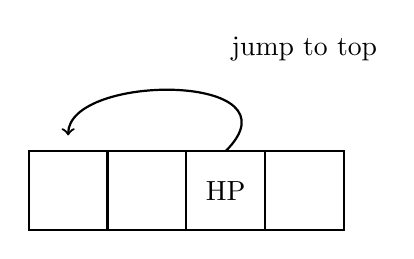
\begin{tikzpicture}
                % Draw the rectangles representing the queue
                \draw[thick] (0,0) rectangle (1,1);
                \draw[thick] (1,0) rectangle (2,1);
                \draw[thick] (2,0) rectangle (3,1);
                \draw[thick] (3,0) rectangle (4,1);
                
                % Arrows to represent "jump to top"
                \draw[->, thick] (2.5, 1) .. controls (3.5, 2) and (0.5, 2) .. (0.5, 1.2);
                
                % Label for high priority
                \node at (2.5, 0.5) {HP};
                
                % Label for "jump to top"
                \node at (3.5, 2.3) {jump to top};
            \end{tikzpicture}
        \end{center}
    \end{definition}

\section{Quicksort (Ch. 7, L10)} % DONE except WS (formal) and AC.
\subsection{Intro}
    \subsubsection{QS algorithm}
    \begin{definition}
        \begin{lstlisting}[language=Python, caption={Quicksort Algorithm Pseudocode}]
            Quicksort (list in, int left, int right)
                pivot = Partition(in, left, right)
                if (pivot > left)
                    Quicksort(in, left, pivot)
                if (pivot < right)
                    Quicksort(in, pivot + 1, right)
        \end{lstlisting}
    \end{definition}

    \begin{intuition}
        \begin{itemize}
            \item \textbf{Quicksort is a divide-and-conquer algorithm:}
            \begin{itemize}
                \item The main idea is to partition the list around a \textbf{pivot element}.
                \item After partitioning, the pivot element is placed in its correct position.
            \end{itemize}
            
            \item \textbf{Steps of Quicksort:}
            \begin{itemize}
                \item \textbf{Choose a pivot element:} This can be the first element, the last element, or any random element in the array.
                \item \textbf{Partitioning:} 
                \begin{itemize}
                    \item Elements smaller than the pivot are moved to the left.
                    \item Elements larger than the pivot are moved to the right.
                \end{itemize}
                \item \textbf{Recursively apply Quicksort:}
                \begin{itemize}
                    \item Apply Quicksort to the subarray to the left of the pivot.
                    \item Apply Quicksort to the subarray to the right of the pivot.
                \end{itemize}
            \end{itemize}
            
            \item \textbf{Base case:}
            \begin{itemize}
                \item When the subarray has one or zero elements, it is already sorted, and no further partitioning is needed.
            \end{itemize}
        \end{itemize}        
    \end{intuition}

    \subsubsection{Partition}
    \begin{definition}
        \begin{lstlisting}[language=Python, caption={Partition Function Pseudocode}]
            int Partition (in, left, right)
                ls = left
                pivot = in(left)
                for i = left + 1 to right
                    if (in(i) <= pivot)
                        ls = ls + 1
                        swap(in(i), in(ls))
                swap(in(left), in(ls))
                return ls
        \end{lstlisting}

        \customFigure[0.5]{00_Images/QS_LS.png}{Partition}
    \end{definition}

    \begin{intuition}
        \customFigure[1]{00_Images/Quicksort_Example1.png}{Quicksort example.}          
    \end{intuition}

\subsection{QS basic analysis}
    \subsubsection{QS best case}
    \begin{derivation}
        The array is always split exactly in half, leading to a balanced partition. The recurrence relation for quicksort in this scenario is:

        \begin{equation*}
            T(n) = 2T\left(\frac{n}{2}\right) + \Theta(n)
        \end{equation*}

        \begin{center}
            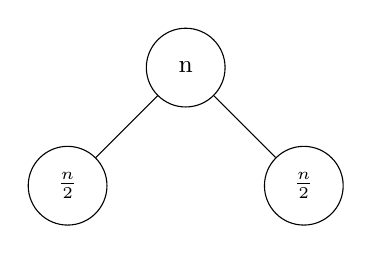
\begin{tikzpicture}[level distance=1.5cm, sibling distance=3cm, every node/.style={circle, draw, minimum size=1cm, font=\small}]
                % Root level for BC
                \node {n}
                    % First level of BC partitioning
                    child {node {$\frac{n}{2}$}}
                    child {node {$\frac{n}{2}$}};
            \end{tikzpicture}
        \end{center}

        \noindent Now using the Master Theorem:
        \begin{equation*}
        T(n) = \Theta(n \log n)
        \end{equation*}
    \end{derivation}

    \subsubsection{QS worst case}
        \begin{derivation}
            The array is already sorted (or reverse sorted) and we choose the first or last element as the pivot, the recurrence relation for quicksort is:

            \[
            T(n) = T(n-1) + \Theta(n)
            \]

            \begin{center}
                % Worst Case (WC) Tree
                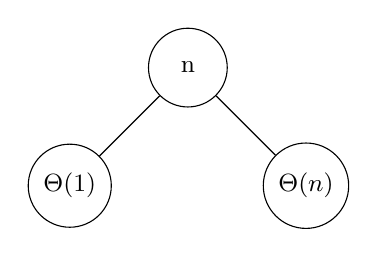
\begin{tikzpicture}[level distance=1.5cm, sibling distance=3cm, every node/.style={circle, draw, minimum size=1cm, font=\small}]
                    % Root level for WC
                    \node {n}
                        % First level of WC partitioning
                        child {node {$\Theta(1)$}}
                        child {node {$\Theta(n)$}};
                \end{tikzpicture}
            \end{center}

            \noindent This recurrence relation expands as follows:

            \begin{align*}
                T(n) &= T(n-1) + \Theta(n) \\
                    &= \left(T(n-2) + \Theta(n-1)\right) + \Theta(n) \\
                    &= \left(T(n-3) + \Theta(n-2)\right) + \Theta(n-1) + \Theta(n) \\
                    &= \cdots \\
                    &= \Theta\left(\sum_{i=1}^{n} i\right) \\
                    &= \Theta\left(\frac{n(n+1)}{2}\right) \\
                    &= \Theta(n^2)
            \end{align*}
        \end{derivation}

    \subsubsection{QS average case}
    \begin{derivation}
        In the average case, the recurrence relation for quicksort can be expressed as:

        \[
        T(n) = T\left(\frac{n}{10}\right) + T\left(\frac{9n}{10}\right) + \Theta(n)
        \]

        \noindent We can visualize this with a recursion tree:

        \customFigure[0.5]{00_Images/Quicksort_Average.png}{Quicksort average case in which each level is derived by subbing in the $T(\#)$ back into the equation above.}          

        \noindent Based on the recursive tree structure and the average-case recurrence relation, we can derive the time complexity as follows:

        \[
        T(n) = h \cdot \Theta(n)
        \]

        \noindent Now, let's calculate the height \( h \) of the tree using the largest element (i.e. right sub-tree):

        \[
        \left(\frac{9}{10}\right)^h n = 1
        \]

        \[
        h = \log_{10/9}(n) 
        \]

        \noindent Substituting this back into the overall complexity:

        \begin{align*}
        T(n) &= h \cdot \Theta(n) \\
            &= \log_{10/9}(n) \cdot \Theta(n) \\
            &= \Theta(n \log n)
        \end{align*}

    \end{derivation}

\subsection{Worst-case (formal)}
    \begin{derivation}
        The worst-case recurrence relation for quicksort can be expressed as:

        \[
        T(n) = \text{time to QS n-elements} = \max_{1 \leq q \leq n-1} \{ T(q) + T(n-q) \} + \Theta(n)
        \]

        \begin{center}
            % Worst Case (WC) Tree
            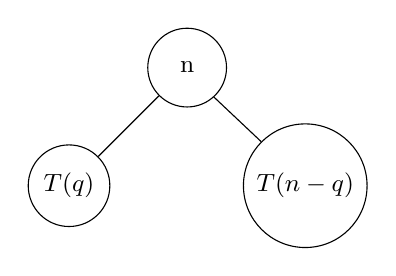
\begin{tikzpicture}[level distance=1.5cm, sibling distance=3cm, every node/.style={circle, draw, minimum size=1cm, font=\small}]
                % Root level for WC
                \node {n}
                    % First level of WC partitioning
                    child {node {$T(q)$}}
                    child {node {$T(n-q)$}};
            \end{tikzpicture}
        \end{center}

        % STOPPED HERE.
        \noindent We use substitution to show that \( T(n) \leq cn^2 \) for some constant \( c \).
        \begin{enumerate}
            \item Guess \( T(n) \leq cn^2 \).
            \item 
        \end{enumerate}
        \begin{align*}
            T(n) &\leq \max_{1 \leq q \leq n-1} \left\{ cq^2 + c(n-q)^2 \right\} + \Theta(n) \quad \text{(Achieves max at } q = 1 \text{ or } q = n-1 \text{)} \\
                 &= c \max_{1 \leq q \leq n-1} \left\{ q^2 + (n-q)^2 \right\} + \Theta(n) \quad \text{(As second derivative is positive (i.e. monotonic), plug } q = 1 \text{)} \\
                 &\leq cn^2 - 2c(n-1) + \Theta(n) \quad \text{(We can pick a large } c \text{ so that } 2c(n-1) \text{ dominates } \Theta(n)) \\
                 &\leq cn^2
        \end{align*}

        \noindent Therefore, using the substitution method, we can show that \( T(n) \leq cn^2 \), confirming that the worst-case time complexity of the quicksort algorithm is \( O(n^2) \).
    \end{derivation}

\subsection{Average-case (formal)}
    \begin{derivation}
        \[
        T(n) = \frac{1}{n} \left( T(1) + T(n-1) + \sum_{z=1}^{n-1} T(z) + T(n-z) \right) + \Theta(n)
        \]

        \begin{itemize}
            \item \textbf{Pivot Small:} $\frac{1}{n} (T(1) + T(n-1)) \leq (\Theta(n^2) + \Theta(1)) \cdot \frac{1}{n} \leq \Theta(n)$
            
            \item \textbf{There are this many elements smaller than the pivot:} $\sum_{z=1}^{n-1} T(z) + T(n-z)$
            
            \item \textbf{Got rid of \( T(1) + T(n-1) \).}
        \end{itemize}
        \vspace{1em}

        Therefore,
        \[
        T(n) \leq \frac{1}{n} \left[ \sum_{q=1}^{n-1} T(q) + T(n-q) \right] + \Theta(n) = \frac{2}{n} \sum_{k=1}^{n-1} T(k) + \Theta(n)
        \]
        \vspace{1em}

        \textbf{Use substitution to prove \( T(n) = a \log(n) + b \) for proper \( a \), \( b \).}
        \begin{enumerate}
            \item Prove the lemma $\sum_{k=1}^{n-1} k \log(k) \leq \frac{1}{2} n^2 \log(n) - \frac{1}{8} n^2$
            \begin{align*}
                \sum_{k=1}^{n-1} k \log(k) &\leq \sum_{k=1}^{\left\lfloor \frac{n}{2} \right\rfloor-1} k \log(k) + \sum_{k=\left\lceil \frac{n}{2} \right\rceil}^{n-1} k \log(k) \\
                &\leq \log \left(\frac{n}{2}\right) \cdot \sum_{k=1}^{\left\lfloor \frac{n}{2} \right\rfloor-1} k + \log(n) \sum_{k=\frac{n}{2}}^{n-1} k \\
                &= \log(n) \sum_{k=1}^{n/2} k - 2 \sum_{k=1}^{n/2} k + \log(n) \sum_{k=n/2}^{n-1} k \\
                &= \log(n) \sum_{k=1}^{n-1} k - 2 \sum_{k=1}^{\left\lceil \frac{n}{2} \right\rceil-1} k \\
                &\leq \frac{1}{2}n(n-1) \log(n) - \frac{1}{2} \left(\frac{n}{2} - 1\right) \cdot \frac{n}{2} \\
                &\leq \frac{1}{2} n^2 \log(n) - \frac{1}{8} n^2
            \end{align*}

            \item Prove using substitution
            \begin{align*}
                T(n) &\leq \frac{2}{n} \sum_{k=1}^{n-1} a k \log(k) + b + \Theta(n) \\
                &\leq a \log(n) - \frac{a}{4n} + 2b + \Theta(n) \\
                &= a n \log(n) + b + \left[\Theta(n) + b - \frac{a}{n} \right] \quad \text{ for large a}
                &\leq an \log(n) + b
            \end{align*}
        \end{enumerate}
    \end{derivation}

\subsection{Randomized QS} 
    \subsubsection{Motivation for randomized QS}
    \begin{example}
        \begin{center}
            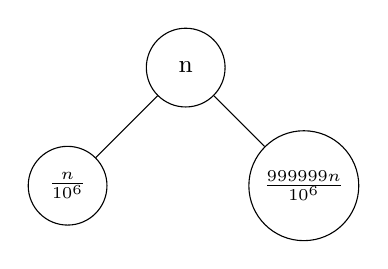
\begin{tikzpicture}[level distance=1.5cm, sibling distance=3cm, every node/.style={circle, draw, minimum size=1cm, font=\small}]
                % Root level
                \node {n}
                    % First level of partitioning
                    child {node {$\frac{n}{10^6}$}}
                    child {node {$\frac{999999n}{10^6}$}};
            \end{tikzpicture}
        \end{center}
        
        \noindent In this example, the array of size \( n \) is split into highly unbalanced sub-arrays:
        \begin{itemize}
            \item One sub-array is \( \frac{n}{10^6} \), very small compared to \( n \).
            \item The other sub-array is \( \frac{999999n}{10^6} \), almost the entire size of \( n \).
        \end{itemize}
        \vspace{1em}

        \noindent This unbalanced split may lead to increased recursion depth and higher running times, potentially reaching the worst-case \( O(n^2) \) complexity.
        \vspace{1em}

        \textbf{Motivation for Randomized QS:}
        \begin{itemize}
            \item Avoiding worst-case scenarios
            \item Ensuring balanced splits
            \item Works against sorted and reverse sorted arrays.
        \end{itemize}
    \end{example}

    \subsubsection{Random partition}
    \begin{definition}
        \begin{lstlisting}[language=Python, caption={Rand-Partition Function Pseudocode}]
            Rand-Partition (list in, left, right)
                i = random(left, right)
                swap(in(left), in(i))
                return Partition(in, left, right)
        \end{lstlisting}
        \begin{itemize}
            \item \textbf{Note:} This partition will be used to find the pivot instead in QS.
        \end{itemize}
    \end{definition}

    \subsubsection{Random partition QS}
    \begin{definition}
        \begin{lstlisting}[language=Python, caption={QuickSort with Random Partition}]
            def QS(C):
                pivot = RAND_partition(C)
                
                if pivot > left:
                    QS(C[left : pivot])
                    
                if pivot < left:
                    QS(C[pivot : right])
            \end{lstlisting}            
    \end{definition}



\section{Counting sort, Radix sort (Ch. 8)}
\subsection{Lower bound on sorting and counting sort}
    \subsubsection{Lower bound on comparison-based sorting}
    \begin{definition}
        No \textbf{comparison-based} sorting algorithm on \textbf{unrestricted} range (i.e. any numbers) can do better than $\Omega(nlog(n))$.    
    \end{definition}

    \subsubsection{Counting sort}
    \begin{definition}
        \begin{lstlisting}[language=Python, caption={Counting Sort Pseudocode}]
            C[i] = 0 for all i in [0...k]
            for j = 1 ... length(A) do  # O(n)
                C[A[j]] = C[A[j]] + 1
            for i = 1 ... k /* prefix sums */ # O(k)
                C[i] = C[i] + C[i-1]
            for j = length(A) ... 1 do # O(n)
                B[C[A[j]]] = A[j]
                C[A[j]] = C[A[j]] - 1 
        \end{lstlisting}
        \begin{itemize}
            \item A: array to be sorted. 
            \item Assume numbers in range $[0...k]$.
            \item Not in-place but stable sorting. 
            \item Time $O(n+k)$ if $O(k) = O(n)$ implies $O(n)$
        \end{itemize}
    \end{definition}




\subsection{Radix sort}
\begin{definition}
    \begin{lstlisting}[language=Python, caption={Radix Sort Pseudocode}]
        for i = Least significant bit (LSB) -> Most significant bit (MSB)
            counting_sort(digit)
    \end{lstlisting}
\end{definition}

\subsubsection{Runtime}
\begin{definition}
    \begin{itemize}
        \item n: \# numbers 
        \item r: range of numbers 
        \item d: \# digits
        \item One pass: $=O(n+r)$
        \item All passes: $dO(n+r) = O(dn + dr)$
        \item If $r=d=O(1)$, then $O(n)$ true.
        \item $1000\#$'s 64 bits. 
        \item Quicksort: $O(nlog(n)) = \frac{O(1000log(1000))}{1000}$
        \item $log(1000) \approx 10$ passes./number
    \end{itemize}
\end{definition}

\section{Selection sort, Binary search trees (Ch. 12)}
\subsection{Selection sort}

\subsection{Binary search trees}

\section{Red black trees (Ch. 13)}
\subsection{Properties}

\subsection{Balance proof}

\subsection{Operations}

\section{Hash tables, Hashing (Ch. 11)}
\subsection{Motivation for Hash Tables}
\begin{intuition}
    In many computer science problems, we need to efficiently solve the \textbf{dictionary problem}, which consists of operations like:
    \vspace{1em}

    \textbf{Dictionary operations:}
    \begin{itemize}
        \item Insert
        \item Search
        \item Delete
        \item Sort (won't be covered in hashing)
    \end{itemize}
    \vspace{1em}

    For instance, storing Social Insurance Numbers (SINs) is an example of a scenario where fast retrieval is essential.

    There are two basic approaches:
    \begin{itemize}
        \item \textbf{Array:} Offers \( O(1) \) search but wastes a lot of memory.
        \item \textbf{Linked List:} Memory efficient $O(n)$ but time inefficient with \( O(n) \) search.
    \end{itemize}

    \customFigure[0.75]{00_Images/HTM.png}{Difference between array and linked lists.}
    \vspace{1em}

    Hash tables offer a tradeoff between these two approaches. Instead of wasting memory like arrays or sacrificing time efficiency like linked lists, hash tables use a hash function to map keys to positions in a table, resolving collisions with methods such as chaining or open addressing.
\end{intuition}

\subsection{Introduction to Hash Tables}

\subsubsection{Definition}
\begin{definition}
A \textbf{hash table} uses a hash function to map keys from the universe of keys \( U \) to positions in an array of size \( m \) called buckets. 
\begin{itemize}
    \item The key is stored in the appropriate bucket. 
    \item The number of keys stored is \( n \).
    \item The \textbf{load factor} \( \alpha \) is given by: $\alpha = \frac{n}{m}, \quad 0 < \alpha \leq 1$
    \begin{itemize}
        \item Expect $n \leq m$ so the places to store in the array is bigger than the number of keys to store in $n$.
    \end{itemize}
\end{itemize}
\end{definition}

\subsubsection{Hash Function}
\begin{definition}
A \textbf{hash function} \( h(\text{key}) \) is used to convert a key into a numeric value, which is then used to index the array. 
\begin{itemize}
    \item i.e. Maps a key in $U$ to an index from $0$ to $m-1$.
    \item A good hash function minimizes collisions, where two or more keys are assigned to the same index.
\end{itemize}
\end{definition}

\begin{example}
    \customFigure[0.75]{00_Images/C.png}{Collisions happening between D and E and also C and F}
    \begin{itemize}
        \item The array goes from $0$ to $m-1$ (i.e. array of size $m$)
        \item The hash function maps the keys from $U$ to the bucket.
        \item Use a linked list for collisions (i.e. resolutions by chaining).
        \item \textbf{Worst-case:} May all hash to the same index. So what constitutes a good hash function. 
    \end{itemize}
\end{example}

\subsection{Method for designing hash functions}
\subsubsection{Modulo}
\begin{definition}
    The modulo operator, denoted as \( \mod \), returns the remainder when one number is divided by another. Specifically, for two integers \( a \) and \( b \), the expression \( a \mod b \) yields the remainder when \( a \) is divided by \( b \).
\end{definition}

\subsubsection{Division Method}
\begin{definition}
    The \textbf{division method} computes the hash as:
    \[
    h(\text{key}) = \text{key} \mod m
    \]
    \begin{itemize}
        \item \( m \) is typically a prime number. 
    \end{itemize}
\end{definition}

\begin{intuition}
    To avoid clustering, \( m \) should be a prime number not too close to a power of 2. This ensures better distribution of keys across the table. 
    \begin{itemize}
        \item Using powers of 2 for \( m \) can lead to poor distributions and clustering. It only considers the lower-order bits of the key, leading to many collisions as different keys may have identical lower bits.

    \end{itemize}
\end{intuition}

\begin{example}
    For example, let \( m = 7 \) and the keys be: 12, 44, 13, 88.
    \[
    h(12) = 12 \mod 7 = 5
    \]
    \[
    h(44) = 44 \mod 7 = 2
    \]
    \[
    h(13) = 13 \mod 7 = 6
    \]
    \[
    h(88) = 88 \mod 7 = 4
    \]

    The array table would be:

    \[
    \begin{array}{|c|c|}
    \hline
    \text{Index} & \text{Key} \\
    \hline
    0 &  \\
    1 &  \\
    2 & 44 \\
    3 &  \\
    4 & 88 \\
    5 & 12 \\
    6 & 13 \\
    \hline
    \end{array}
    \]
\end{example}

\subsubsection{Multiplication Method}
\begin{definition}
The \textbf{multiplication method} computes the hash as:
\[
h(\text{key}) = \left\lfloor m \cdot ((\text{key} \cdot A) \mod 1) \right\rfloor
\]
\begin{itemize}
    \item \( A = \frac{\sqrt{5} - 1}{2} \), the golden ratio, is used to spread keys more evenly. 
    \item $m = 2^p$ are good values.  
\end{itemize}
\end{definition}

\begin{example}
        The multiplication method computes the hash function as: 
    \[
    h(\text{key}) = \lfloor m \cdot ((\text{key} \cdot A) \mod 1) \rfloor
    \]
    where \( A \approx 0.6180339887 \) and \( m = 16 \).

    For example, with keys 123, 456, 789, 102, the hash values are:

    \[
    \begin{array}{|c|c|}
    \hline
    \text{Index} & \text{Key} \\
    \hline
    0 & 123, 102 \\
    1 &  \\
    2 &  \\
    3 &  \\
    4 &  \\
    5 &  \\
    6 &  \\
    7 &  \\
    8 &  \\
    9 &  \\
    10 & 789 \\
    11 &  \\
    12 &  \\
    13 & 456 \\
    14 &  \\
    15 &  \\
    \hline
    \end{array}
    \]    
\end{example}

\subsubsection{Universal Hashing}
\begin{definition}
In \textbf{universal hashing}, a family of hash functions \( H = \{ h_1, h_2, h_3, \ldots \} \) is randomly chosen from. The key advantage is that it reduces the probability of collisions between specific sets of keys.
\end{definition}

\subsection{Resolution by Chaining}
\begin{definition}
\textbf{Chaining} is a method of resolving collisions by maintaining a linked list at each bucket. If two or more keys hash to the same index, they are stored in the same linked list.
\end{definition}

\begin{intuition}
Chaining is simple and can easily handle cases where multiple keys collide by inserting them into the linked list of the corresponding bucket. The downside is that it can lead to increased search time if the linked lists become long.
\end{intuition}

\subsection{Resolution by Open Addressing}

\begin{definition}
\textbf{Open addressing} resolves collisions by probing for the next available slot in the table. 
\begin{itemize}
    \item Instead of maintaining a list of keys at each bucket, each key is placed directly in the table, and a probing sequence is followed if collisions occur.
\end{itemize}
\end{definition}

\subsubsection{Probing Methods}
\begin{definition}
    \begin{itemize}
        \item \textbf{Linear Probing:} Probe and insert next element:
        
        \[
        L_0 = h(\text{key})
        \]
        
        If bucket is full (i.e. collision), then we check the next slot in the table until an empty one is found (i.e. reprobe)
        \[
        L_{j+1} = (L_j + 1) \mod m
        \]
        \begin{itemize}
            \item However, linear probing can lead to \textbf{clustering}, where groups of keys form large contiguous blocks in the array.
        \end{itemize}
        \customFigure[0.5]{00_Images/Cl.png}{Clustering}
    
        \item \textbf{Double Hashing:} Using two hash functions to avoid clustering. If a collision occurs at index \( i_0 \):
        \[
        L_1 = h_1(\text{key}) 
        \]
        The next probe location is computed by:
        \[
        L_{j+1} = (L_j + h_2(\text{key})) \mod m
        \]
        \begin{itemize}
            \item This results in better distribution of keys across the table and reduces clustering.
        \end{itemize}
    \end{itemize}
\end{definition}

\begin{example}
    Example of linear probing:
    \textbf{Given:}
    \begin{itemize}
        \item Hash table size, $m = 7$
        \item Probe step size, $c = 3$
        \item Hash function: $h(\text{key}) = \text{key} \mod 7$
        \item Keys to insert: \{14, 8, 21, 10\}
    \end{itemize}
    
    \textbf{Insertion of Keys:}
    \begin{enumerate}
        \item \textbf{Insert 14}:
           \[
           h(14) = 14 \mod 7 = 0
           \]
           Place 14 at index 0.
    
        \item \textbf{Insert 8}:
           \[
           h(8) = 8 \mod 7 = 1
           \]
           Place 8 at index 1.
    
        \item \textbf{Insert 21}:
           \[
           h(21) = 21 \mod 7 = 0
           \]
           Collision at index 0 (occupied by 14).  
           Perform linear probing with step size 3:
           \[
           \text{Next index} = 0 + 3 = 3
           \]
           Place 21 at index 3.
    
        \item \textbf{Insert 10}:
           \[
           h(10) = 10 \mod 7 = 3
           \]
           Collision at index 3 (occupied by 21).  
           Perform linear probing with step size 3:
           \[
           \text{Next index} = 3 + 3 = 6
           \]
           Place 10 at index 6.
    \end{enumerate}
    
    \textbf{Current Hash Table:}
    
    \[
    \begin{array}{|c|c|}
    \hline
    \text{Index} & \text{Value} \\
    \hline
    0 & 14 \\
    1 & 8 \\
    2 & - \\
    3 & 21 \\
    4 & - \\
    5 & - \\
    6 & 10 \\
    \hline
    \end{array}
    \]
    
    \textbf{Deletion of Keys:}
    \begin{enumerate}
        \item \textbf{Remove 21}:
           \[
           h(21) = 0
           \]
           Check index 0: Not 21.  
           Perform linear probing:
           \[
           \text{Next index} = 0 + 3 = 3
           \]
           Find 21 at index 3, remove it, and place a tombstone at index 3.
    
        \item \textbf{Remove 10}:
           \[
           h(10) = 3
           \]
           Check index 3: Tombstone.  
           Perform linear probing:
           \[
           \text{Next index} = 3 + 3 = 6
           \]
           Find 10 at index 6 and remove it.
    \end{enumerate}
    
    \textbf{Final Hash Table:}
    
    \[
    \begin{array}{|c|c|}
    \hline
    \text{Index} & \text{Value} \\
    \hline
    0 & 14 \\
    1 & 8 \\
    2 & - \\
    3 & \text{Tombstone} \\
    4 & - \\
    5 & - \\
    6 & \text{Tombstone} \\
    \hline
    \end{array}
    \]
    
    \textbf{Explanation:} Tombstones are used in open addressing to indicate that an element was removed from that position. If a tombstone is found during probing, the search continues, ensuring that other elements inserted with probing can still be located.
    
\end{example}

\subsection{Load Factor in Open Addressing and Chaining}
\begin{definition}
    The expected search time (i.e. expected number of probes) depends on the load factor \( \alpha \) and the probing method used:
    \begin{itemize}
        \item Deteriorates as $\alpha$ increases because it increases the number of collisions (i.e. more probes required).
    \end{itemize}

    \begin{itemize}
        \item \textbf{Linear Probing:} 
        \[
        \text{\# Probes} = \frac{1}{2} \left( 1 + \frac{1}{1 - \alpha} \right)
        \]
        \item \textbf{Double Hashing:} 
        \[
        \text{\# Probes} = \frac{1}{\alpha} \ln \left( \frac{1}{1 - \alpha} \right) \approx O(1) \text{ if } n<m
        \]
        \item \textbf{Chaining:}
        \[
            \text{\# Probes} = 1 + \frac{\alpha}{2}
            \]
    \end{itemize}
    \begin{itemize}
        \item \textbf{Note:} The number of collisions is the number of probes.
    \end{itemize}
\end{definition}

\begin{intuition}
    Chaining (blue), linear probing (red), double hashing (green)

    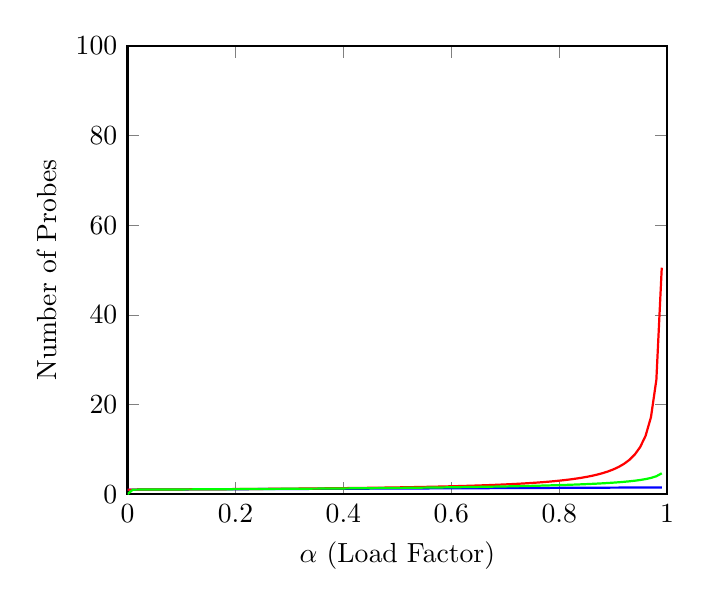
\begin{tikzpicture}
        \begin{axis}[
            xlabel={$\alpha$ (Load Factor)},
            ylabel={Number of Probes},
            xmin=0, xmax=1,
            ymin=0, ymax=100,
            domain=0:0.99,
            samples=100,
            thick
        ]
        
        % Chaining
        \addplot[
            color=blue,
            solid,
        ]{1 + x/2};
    
        % Linear Probing
        \addplot[
            color=red,
            solid,
        ]{0.5*(1 + 1/(1-x))};
    
        % Double Hashing
        \addplot[
            color=green,
            solid,
        ]{(1/x)*ln(1/(1-x))};
        \end{axis}
    \end{tikzpicture}    
\end{intuition}


\section{Dynamic programming (Ch. 14)}
\subsection{Intro to dynamic programming}
\begin{definition}
    Dynamic programming is an epitome of the "divide and conquer" approach. It often deals with max/min problems, utilizing two key characteristics:
    \begin{enumerate}
        \item \textbf{Optimal substructure:} Break problem into smaller problems of same nature, find solutions to subproblems and combine results 
        \item \textbf{Overlapping subproblems:} The same subproblems are solved multiple times, which can be avoided using \textit{memoization} to store/retrieve the intermediate results.
    \end{enumerate}
\end{definition}

\begin{example}
    Motivation for memoization:
    \begin{equation*}
        f_0 = 0, \quad f_1 = 1, \quad f_i = f_{i-1} + f_{i-2}
        \end{equation*}
        
        For example, consider calculating \(F(100)\):
        
        \customFigure[0.5]{00_Images/S.png}{Fib numbers}
        
        \begin{itemize}
            \item \textbf{Solution:} Notice that during the calculation of \(F(99)\) and \(F(98)\), \(F(98)\) is calculated more than once. Hence, it is efficient to store the computed values in an array and access them directly instead of recalculating (i.e. memoization).
        \end{itemize}
\end{example}

\subsection{DP matrix multiplication}
\subsubsection{Optimal Matrix Parenthesization Problem Setup}
\begin{definition}
    Given matrices \(A_1, A_2, \dots, A_n\), we seek the optimal way to multiply them in that order that minimizes the number of scalar multiplications. 
\end{definition}

\begin{intuition}
Matrix multiplication is associative, but the order in which matrices are multiplied affects the number of operations. The goal is to find the optimal parenthesization that minimizes this count.
\end{intuition}

\begin{example}
    Consider the matrices
    \[
    A_1 \in \mathbb{R}^{10 \times 100}, \quad A_2 \in \mathbb{R}^{100 \times 5}, \quad A_3 \in \mathbb{R}^{5 \times 50}
    \]
    We need to find the minimum cost of multiplying \(A_1 A_2 A_3\).
    \vspace{1em}

    Possible parenthesizations and their associated costs:
    \[
    (A_1 A_2) A_3 = (10 \times 100 \times 5) + (10 \times 5 \times 50) = 7500
    \]
    \begin{itemize}
        \item \textbf{First Term:} $A_1 A_2$: $10 \times 100 \times 5$
        \item \textbf{Second Term:} $(A_1 A_2) \in \mathbb{R}^{10 \times 5}$, so $(A_1 A_2) A_3$: $10 \times 5 \times 50$.
    \end{itemize}
    \vspace{1em}

    \[
    A_1 (A_2 A_3) = (100 \times 5 \times 50) + (10 \times 100 \times 50) = 75000
    \]
    \begin{itemize}
        \item \textbf{First Term:} $A_2 A_3$: $ 100 \times 5 \times 50$
        \item \textbf{Second Term:} $(A_2 A_3) \in \mathbb{R}^{100 \times 500}$, so $(A_1 A_2) A_3$: $100 \times 500 \times 50$
    \end{itemize}
    Thus, the optimal solution is to compute \((A_1 A_2) A_3\) with a cost of 7500 scalar multiplications.
\end{example}

\subsubsection{Total number of parenthesization}
\begin{definition}
    The total number of possible parenthesizations for multiplying \(A_1, A_2, \dots, A_n\):

    \begin{equation*}
    \text{Total number of parenthesizations} = \sum_{k=1}^{n-1} P(k)P(n-k) = \Omega \left(\frac{4^n}{n^{3/2}}\right) 
    \end{equation*}
    \begin{itemize}
        \item \textbf{Note:} The solution is given since we don't know hwo to solve the reccurrence. 
        \item \textbf{Key:} Therefore the brute force method of calculating all the parenthesizations and finding the minimum amount is non-trivial due to when $n\rightarrow \infty$.
    \end{itemize}
   
\end{definition}

\subsubsection{Recursive Formula for Cost}
\begin{definition}
    Let matrix \(A_i = P_{i-1} \times P_i\) denote the dimensions of the matrix, and let \(A_{ij} = A_i \cdots A_j\) represent the product of matrices from \(i\) to \(j\).
    \vspace{1em}

    The recursive formula for the minimal cost \(m(i,j)\) (i.e. optimal number of SM to evaluate matrices \(A_i \dots A_j\)) is given by:

    \begin{equation*}
    m(i,j) = 
    \begin{cases}
    0 & \text{if} \quad i = j \\
    \min_{i \leq k < j} \left( m[i,k] + m[k+1,j] + P_{i-1} P_k P_j \right) & \text{if} \quad i < j
    \end{cases}
    \end{equation*}
    \begin{itemize}
        \item \textbf{Purpose:} Find the optimal substructure (i.e. first principle of dynamic programming)
        \item \textbf{Intuition:} Find which $k$ minimizes the SM of the matrices on the left of $k$ and the right of $k$, which is $m[i,k]$ (left) $m[k+1,j]$ (right). The final term \(P_{i-1} P_k P_j\) comes from multiplying $m[i,k]$, and $m[k+1,j]$ together. 
        \begin{itemize}
            \item $A_1 A_2 \cdots A_i \cdots A_k A_{k+1} \cdots A_j \cdots A_{n-1} A_n$
            \begin{itemize}
            \item $A_i \cdots A_k = A_{ik}$ and $A_{k+1} \cdots A_j = A_{(k+1)j}$
            \end{itemize}
        \end{itemize} 
    \end{itemize}
\end{definition}

\subsubsection{Why is the first principle (i.e. optimal substructure) not sufficient?}
\begin{example}

    \customFigure[0.75]{00_Images/EX1.png}{Why memoization is needed}

    \begin{itemize}
        \item \textbf{Note:} This recursive pattern is similar to the approach used for Fibonacci sequence calculations, highlighting overlapping subproblems. So memoization is needed.
        \begin{itemize}
            \item \textbf{Store:} Store the results in a 2D array since we have two different indices $i$ and $j$.
        \end{itemize}
    \end{itemize}
\end{example}

\subsubsection{Matrix Chain Multiplication Example}
\begin{example}
    Consider the matrices with the following dimensions:

    \[
    A_1: 30 \times 35, \quad A_2: 35 \times 15, \quad A_3: 15 \times 5, \quad A_4: 5 \times 10, \quad A_5: 10 \times 20, \quad A_6: 20 \times 25
    \]

    The goal is to find the minimum cost of multiplying these matrices together and store them in a 2D result.
    \vspace{1em}

    The triangle below represents the minimum number of scalar multiplications needed for each subproblem. Each entry in the triangle corresponds to the cost of multiplying the matrices from \(A_i\) to \(A_j\). 

    \customFigure[0.5]{00_Images/M.png}{You do not need the whole 2D array, you just need the upper triangle of the 2D array. Calculate this table from the bottom up.}
    \begin{itemize}
        \item \textbf{Key:} $\text{cell}(i,j)$ holds $m(i,j)$.
        \item \textbf{Bottom Row:} All zeros because there is no scalar multiplication when $i=j$ (i.e. same matrix)
        \item \textbf{1-2}: $30 \times 35 \times 15$
        \item \textbf{1-3} $A_1 A_2 A_3$ either with $(A_1 A_2)A_3$ and $A_1 (A_2A_3)$
        \begin{itemize}
            \item $(A_1 A_2)A_3$: $15750 + 30 \times 15 \times 5$
            \item $A_1 (A_2A_3)$: $2625 + 30 \times 35 \times 5$ (this one is smaller), so $m(1,3)$ is this. 
            \begin{itemize}
                \item \textbf{Note:} Use an arrow to denote from which bottom row is made.  
            \end{itemize}
        \end{itemize}
        \item \textbf{1-4}: We will now calculate the cost for multiplying a subset of the matrices $A_1 A_2 A_3 A_4$.
        \begin{enumerate}
            \item First, consider multiplying \(A_1[A_2 A_3 A_4]\):
            \[
            = 4375 + (30 \times 35 \times 10) = 4375 + 10500 = 14875
            \]
            \item Now, consider multiplying \([A_1 A_2][A_3 A_4]\):
            \[
            = 15750 + 750 + (30 \times 15 \times 10) = 15750 + 750 + 4500 = 21000
            \]
        
            \item Finally, consider multiplying \([A_1 A_2 A_3] A_4\):
            \[
            = 7875 + (30 \times 5 \times 10) = 7875 + 1500 = 9375
            \]
        \end{enumerate}
        \begin{itemize}
            \item \textbf{Note:} This is made easier using memoization.
        \end{itemize}
        Thus, the optimal solution $m(1,4)$ for multiplying \(A_1 A_2 A_3 A_4\) is \(9375\) scalar multiplications.
    \end{itemize}
    \vspace{1em}
\end{example}

\subsubsection{Time Complexity}
\begin{definition}
    The time complexity of this algorithm is determined by the number of subproblems (or squares in the table), leading to a total complexity of:

    \[
    n \mathcal{O}(n^2) = \mathcal{O}(n^3)
    \]
    \begin{itemize}
        \item \textbf{Note:} where \(n\) is the index since the index can go up to $n$ times for $m(i,j)$ since we have to find the lowest one. 
    \end{itemize}
\end{definition}

\subsection{DP longest common subsequence (LCS)}
\begin{definition}
Given two strings \(X = x_1, x_2, \dots, x_m\) and \(Y = y_1, y_2, \dots, y_n\), the longest common subsequence (LCS) of \(X\) and \(Y\) is the longest sequence that appears in both strings in the same order, though not necessarily consecutively.
\begin{itemize}
    \item \textbf{Notation:} Let \(X^k = x_1, x_2, \dots, x_k\) denote a substring of \(X\).
\end{itemize}
\end{definition}

\begin{example}
    Springtime and pioneer. pine is the LCS.
\end{example}

\begin{intuition}
    \textbf{Naive approach:} Assuming \(n > m\), a brute force solution has a time complexity of \(\Omega(m^2 n^2)\).
\end{intuition}

\begin{theorem}
If \(Z = z_1, z_2, \dots, z_k\) is the LCS of \(X\) and \(Y\), then:
\begin{itemize}
    \item[(A)] If \(x_m = y_n\), then \(x_m = y_n = z_k\) and \(z_{k-1}\) is the LCS of \(X_{m-1}\) and \(Y_{n-1}\).
    \item[(B)] If \(x_m \neq y_n\), then \(z_k \neq x_m\), so \(Z\) is the LCS of \(X_{m-1}\) and \(Y_n\).
    \item[(C)] If \(x_m \neq y_n\), then \(z_k \neq y_n\), so \(Z\) is the LCS of \(X_m\) and \(Y_{n-1}\).
\end{itemize}
\end{theorem}

\begin{derivation}
    \textbf{Proof of (A):}
    \begin{enumerate}
        \item ATaC that \(x_m = y_n\) and \(x_m = y_n = z_k\), but \(Z_{k-1}\) is not the LCS of \(X_{m-1}\) and \(Y_{n-1}\). 
        \item As a result, some other string \(W\) would be the LCS, implying \(|W| \cup z_k > |Z_{k-1}| \cup z_k = Z\), which contradicts the assumption that \(Z\) is the longest common subsequence. 
    \end{enumerate}
    \begin{itemize}
        \item (B) and (C) follow similarly by considering the cases where \(x_m \neq y_n\).
    \end{itemize}
\end{derivation}

\begin{intuition}
If the last characters of \(X\) and \(Y\) match, they are part of the LCS. Otherwise, we reduce the problem by eliminating the last character of either \(X\) or \(Y\) and finding the LCS of the reduced strings.
\end{intuition}

\subsubsection{Dynamic Programming Approach}
\begin{definition}
    We define \(C[i, j]\) as the length of the LCS of \(X_i\) and \(Y_j\).

    \begin{equation}
    C[i, j] = 
    \begin{cases}
    0 & \text{if} \quad i = 0 \quad \text{or} \quad j = 0 \\
    C[i-1, j-1] + 1 & \text{if} \quad x_i = y_j \quad \text{(case A)} \\
    \max(C[i-1, j], C[i, j-1]) & \text{if} \quad x_i \neq y_j \quad \text{(cases B, C)}
    \end{cases}
    \end{equation}

\end{definition}

\begin{intuition}
    
\end{intuition}

\begin{example}
Consider the strings \(X = \text{computer}\) and \(Y = \text{automation}\). The dynamic programming table for \(C[i,j]\) is shown below.

\customFigure[0.5]{00_Images/LCS.png}{Computation of C}

WHAT DOES THAT FIGURE MEAN IN THE RIGHT ON WEEBLY.
\end{example}

\subsubsection{Time Complexity}
\begin{definition}
    The time complexity of this approach is \(\mathcal{O}(m \times n)\)
    \begin{itemize}
        \item \(m\) is the length of string \(X\)
        \item \(n\) is the length of string \(Y\). 
        \item \textbf{Note:} The algorithm fills a table of size \(m \times n\), and for each cell, it performs a constant number of operations.
    \end{itemize}
\end{definition}

\subsubsection{Recursive Formula for Binomial Coefficient}
\begin{definition}
    \begin{equation}
        C(n,k) = \binom{n}{k}
    \end{equation}
        
        The base cases are:
        \[
        C(n, 0) = 1, \quad C(n, n) = 1
        \]
        The recursive relation is:
        \[
        C(n, k) = C(n-1, k-1) + C(n-1, k)
        \]
\end{definition}

\subsection{Optimal Polygon Triangulation FINISH IN LEC}

\begin{definition}
    Given a convex polygon with \(n\) vertices \(v_1, v_2, \dots, v_n\), triangulation is the division of the polygon into triangles by adding diagonals. The goal is to find the triangulation that minimizes the total weight \(\omega\).
\end{definition}
    
\subsubsection{Objective}
\begin{definition}
    Minimize the total weight of the triangulation, where the weight \(\omega(\Delta v_i v_j v_k)\) of a triangle is the sum of the Euclidean distances between its vertices:
    \begin{equation}
        \omega(\Delta v_i v_j v_k) = |v_i v_j| + |v_j v_k| + |v_i v_k|
    \end{equation}
\end{definition}    

\subsubsection{Recursive formula}
\begin{definition}
    The recursive formula for the optimal triangulation of vertices \(v_i \dots v_j\) is given by:
    
    \begin{equation}
    t[i, j] = 
    \begin{cases}
    0 & \text{if} \quad i = j \\
    \min_{i \leq k \leq j} \left( t[i, k] + t[k+1, j] + \omega(\Delta v_i v_j v_k) \right) & \text{if} \quad i < j
    \end{cases}
    \end{equation}
\end{definition}

\textbf{Triangulation as a tree:} The triangulation can be represented as a binary tree structure, where each node corresponds to a triangle, and the optimal triangulation is achieved by recursively minimizing the weights of the subproblems.
    
\[
\begin{array}{ccccccccc}
v_0 & v_1 & v_2 & v_3 & v_4 & v_5 & v_6 \\
\end{array}
\]
\[
\begin{array}{c}
\underbrace{\hspace{1.5cm}}_{\text{Triangulation of } v_0 \dots v_3} \hspace{1cm} \underbrace{\hspace{1.5cm}}_{\text{Triangulation of } v_4 \dots v_6}
\end{array}
\]
    
    \textbf{Example:} The optimal triangulation of vertices \(v_1 \dots v_6\) can be represented as:
    
    \[
    ((((v_0 v_1 v_2) v_3) v_4) (v_5 v_6))
    \]
    
    This recursive structure can be visualized as a tree, with the leaves representing the individual triangles and the root representing the entire polygon.

\customFigure[0.75]{00_Images/PT.png}{Polygon triangulation.}

\section{Greedy algorithms (Ch. 15)} % MIDTERM CUT
\subsection{Greedy Algorithms Intro and Class Scheduling}

\begin{intuition}
    \begin{itemize}
        \item "Greed works, greed is right, greed is good." 
        \item Greedy algorithms make locally optimal choices at each stage with the goal of finding a global optimum. This approach can approximate NP-complete problems.
    \end{itemize}
\end{intuition}

\subsubsection{Characteristics}
\begin{intuition}
        \begin{itemize}
            \item Optimal substructure
            \item Greedy principle: a greedy choice now leads to a global optimum
        \end{itemize}
\end{intuition}

\subsubsection{Class Scheduling Example}
\begin{example}
    Given one room and many classes, the goal is to maximize the number of classes scheduled in one day. 
    \begin{itemize}
        \item Sort by finish time.
        \item Schedule classes in order based on sorted times.
    \end{itemize}
    \customFigure[0.75]{00_Images/CSE.png}{Class scheduling example.}
    The time complexity for sorting is $O(n\log(n))$.
\end{example}

\subsubsection{Proof of Correctness of Class Scheduling (On exams)}
\begin{derivation}
    \begin{itemize}
        \item ATaC: Given that greedy choices $g_1, g_2, \dots, g_n$ are not optimal, but some other optimal choices $o_1, o_2, \dots, o_m$ exist $(m > n)$. 
        \item By the way the greedy algorithm works, $f(g_i) \leq f(o_i)$ (f is the finish time) because it replaces based on the finish time. 
        \customFigure[0.75]{00_Images/POC.png}{WHAT IS THIS EXAMPLE SHOWING.}
        \item $o_{n+1},\dots, o_m$ cannot exist as greedy algorithm would take these into account, therefore, this implies a contradiction since the greedy algorithm would take these into account.
    \end{itemize}
\end{derivation}

\subsection{Knapsack Problem}

\subsubsection{Problem setup}
\begin{intuition}
A thief breaks into a store and the thief's bag can carry up to $\omega$ weight. The store has $n$ items, each with weight $w_i$ and value $v_i$ of item $i$.
\end{intuition}

\subsubsection{Types of Knapsack Problems}
\begin{definition}
    \begin{itemize}
        \item \textbf{Fractional:} Can take part of an item (Greedy solution).
        \item \textbf{0-1:} Can take or not take an item (Dynamic programming).
    \end{itemize}
\end{definition}

\subsubsection{Fractional Knapsack}
\begin{definition}
For fractional knapsack:
\begin{itemize}
    \item Sort $\frac{v_i}{w_i}$ and keep taking items in that order.
\end{itemize}
\end{definition}

\subsubsection{0-1 Knapsack}
\begin{definition}
    For 0-1 knapsack, fix some order $1, \dots, n$ of the items. The recursive formula for 0-1 knapsack is:
    \[
    C[i, \omega] = \begin{cases} 
        0 & \text{if } i = 0, \omega = 0 \\
        C[i-1, \omega] & \text{if } w_i > \omega \\
        \max \{C[i-1, \omega - \omega_i] + v_i, \; C[i-1, \omega]\} & \text{if } \omega \geq \omega_i 
    \end{cases}
    \]
    where $C[i, \omega]$ denotes the maximum value achievable with $i$ items and a leftover weight of $\omega$.
\end{definition}

\subsection{Intro to Huffman Encoding}
\begin{intuition}
    \customFigure[0.75]{00_Images/I.png}{WHAT IS THIS SHOWING ME }
    \begin{itemize}
        \item 
    \end{itemize}
\end{intuition}

\subsubsection{Problem Statement}
\begin{intuition}
Huffman coding minimizes the size of the encoded file by assigning fewer bits to more frequent characters.
\begin{equation*}
    \sum_c f(c)d(c) = \text{total number of bits needed.}
\end{equation*}
\end{intuition}

\begin{example}
    \customFigure[0.75]{00_Images/CHARS.png}{WHAT IS THIS SHOWING ME?}
    \begin{itemize}
        \item 
    \end{itemize}
\end{example}

\subsubsection{Steps in Huffman Coding}
\begin{itemize}
    \item Write two letters with the lowest frequency in a tree-like fashion.
    \item Replace the two letters with a new character that sums their frequencies.
    \item Label the resulting tree.
    \customFigure[0.75]{00_Images/LG.png}{Tree}
\end{itemize}

\subsubsection{Proof of Correctness}
\begin{theorem}
Every optimal tree can have the two lowest frequency keys being siblings, that differ only on one bit, with the greatest depth.

\end{theorem}

IS THIS A PROOF?
\begin{derivation}
    Assume two lowest frequency keys $x$ and $y$ and $T''$ remains optimal. 
    \customFigure[0.75]{00_Images/E.png}{T optimal, T', and T''}
    \vspace{1em}

    \begin{enumerate}
        \item Let $B(T)$ be the sum of the frequencies and their bit-lengths:
        \[
        B(T) = \sum_c f(c) \cdot d(c)
        \]
        We want to show that $B(T') \leq B(T_{\text{opt}})$, where $T_{\text{opt}}$ is the optimal tree and $T'$ is a different tree (similar proof for $B(T'') \leq B(T')$)
        \vspace{1em}
    
        \item By the greedy principle:
        \[
        B(T_{\text{opt}}) - B(T') = \sum_c f(c)(d(c_{opt}) - \sum_c f(c) d(c_{gr}) \geq 0
        \]
        Thus, $B(T_{\text{opt}}) \geq B(T')$.
    \end{enumerate}
\end{derivation}

\subsubsection{Optimal Substructure}
WHAT IS THE WORKFLOW, HOW DID WE GET HERE. IS THIS A THEOREM?
\begin{theorem}
    \begin{enumerate}
        \item Let \( x \) $\leftarrow z \rightarrow$ \( y \) be part of \( T_{\text{opt}} \) for character set \( C \). Then
        \[
        T_{\text{opt}} = T_{\text{opt}} - \{x, y\} + \{z\}
        \]
        is optimal prefix code for new set \( C' = C - \{x, y\} + \{z\} \), where \( f(z') = f(x) + f(y) \).
    
        \item We have
        \[
        f(x) \cdot d_{T_{\text{opt}}}(x) + f(y) \cdot d_{T_{\text{opt}}}(y) = f(z) \cdot d_{T_{\text{opt}}}(z) + [f(x) + f(y)]
        \]
        because 
        \[
        d_{T_{\text{opt}}}(x) = d_{T_{\text{opt}}}(y) = d_{T_{\text{opt}}}(z) + 1.
        \]
    
        \item Every time we "move" from \( T_{\text{opt}} \) to \( T'_{\text{opt}} \) by merging 2 keys, we have
        \[
        \mathcal{B}(T_{\text{opt}}) = \mathcal{B}(T'_{\text{opt}}) + (f(x) + f(y)).
        \]
    
        \item ATaC \( T'_{\text{opt}} \) is not optimal for \( C' \), but \( T'' \) is. 
    
        \[
        \mathcal{B}(T'') + (f(x) f(y)) < \mathcal{B}(T'_{\text{opt}}) + (f(x) f(y)),
        \]
        which is more optimal than \( T_{\text{opt}} \), a contradiction.
    \end{enumerate}

\end{theorem}

\section{Amortized analysis (Ch. 16)}
\begin{definition}
A worst-case guarantee (bound) for the average case. We view/analyze every operation as part of the sequence of $n$ operations. If $n$ operations take $T(n)$ time, the operation has $T(n)/n$ amortized costs, which may be different from the actual cost.
\end{definition}

\subsubsection{Analysis Methods}
\begin{itemize}
    \item Aggregate method (brute force)
    \item Accounting method (splay).
    \item Potential method.
\end{itemize}

\subsubsection{Stack Operations}
\begin{itemize}
    \item \textbf{Push:} $O(1)$
    \item \textbf{Pop:} $O(1)$ (naive: $O(n)$ if we call multipop $n$ times)
    \item \textbf{Multipop:} $O(n)$
\end{itemize}

\begin{warning}
    You cannot pop more than what you push, hence $n$ operations can take at most $O(n)$ time or $O(n)/n$ amortized time.
\end{warning}

\subsubsection{Binary Counter: Increment}
\begin{lstlisting}
Increment(A, k)
    i = 0
    while i < k and A[i] == 1:
        A[i] = 0
        i = i + 1
    if i < k:
        A[i] = 1
\end{lstlisting}

\begin{warning}
    Let $k = n$. Assume $O(1)$ to flip $1 \rightarrow 0$ or $0 \rightarrow 1$. Increment is $O(n)$ time $\Rightarrow$ calling $n$ times is $O(n^2)$.
\end{warning}

\subsubsection{Aggregate Analysis of Flips}
\begin{definition}
    \[
\# \text{ bit flips} = \sum_{i=0}^{n} \frac{n}{2^i}
\]
The total bit flips is $\leq 2n$, and the amortized cost of increment is $O(1)$.
\end{definition}


\subsubsection{Accounting Method}
\begin{definition}
We charge \$ for every operation, and the data structure behaves like a ``bank".
\begin{itemize}
    \item \textbf{Amortized cost} $=$ what we charge.
    \item \textbf{Actual cost} $=$ how expensive the operation actually is.
    \item If amortized cost $>$ actual cost $\Rightarrow$ save/deposit on the data structure.
    \item If amortized cost $<$ actual cost $\Rightarrow$ use credit from the data structure.
    \item We cannot run during analysis on negative credit.
\end{itemize}
\end{definition}

\subsubsection{Stack Operations Table}

\begin{table}[h!]
\centering
\begin{tabular}{|c|c|c|}
\hline
Operation & Actual Cost & Amortized Cost \\
\hline
Push & $O(1)$ & \$2 \\
Pop & $O(1)$ & \$1 \\
Multipop & $O(n)$ & \$0 \\
\hline
\end{tabular}
\caption{Cost table for stack operations}
\end{table}

For $n$ operations, we need $2n$ or $O(n)/n = O(1)$ in an amortized sense.

\section{Splay trees}
\begin{definition}
    Splay trees are binary search trees (BSTs) without any structural balancing condition. 
    \begin{itemize}
        \item \textbf{Weighted dictionary problem:} Key and frequencies accessed. You want to insert, delete, and search.
    \end{itemize}
\end{definition}

\subsection{Online vs. Offline:}
\begin{definition}
    \begin{itemize}
        \item \textbf{Offline:} A prior know the frequencies.
        \item \textbf{Online:} Splay trees achieve the info $\rightarrow$ achieves theoretical optimality (amortized sense) 
    \end{itemize}
\end{definition}


\subsection{Splay operation}
\begin{definition}
    \begin{lstlisting}
        Splay(x):
            while x != root:
                if p(x) = root: # zig
                    rotate p(x)
                if p(x) and x both left or both right child: # zigzig
                    rotate p(p(x))
                    rotate p(x)
                else: # zigzag
                    rotate p(x)
                    rotate p(p(x))
    \end{lstlisting}
\end{definition}

\begin{intuition}
    \begin{enumerate}
        \item \textbf{Zig Case}: 
        \begin{lstlisting}
        Occurs when x's parent is the root.
        - Intuition: x is one step from the root, so a single rotation is enough to bring x to the root.
        \end{lstlisting}
    
        \item \textbf{Zig-Zig Case}: 
        \begin{lstlisting}
        Occurs when both x and its parent are on the same side (both left or both right).
        - Intuition: Two aligned nodes, so we perform two rotations in the same direction to bring x closer to the root.
        \end{lstlisting}
    
        \item \textbf{Zig-Zag Case}:
        \begin{lstlisting}
        Occurs when x and its parent are on opposite sides (one left, one right).
        - Intuition: Zig-zag structure is flattened by alternating two rotations in opposite directions.
        \end{lstlisting}
        
    \end{enumerate}  
\end{intuition}

\begin{example}
    \customFigure[0.75]{00_Images/EX2.png}{Example 2}
\end{example}

\subsection{Operations}
\begin{definition}
    \begin{itemize}
        \item \textbf{Search(x):} Like BST and splay $x$. $O(\log n)$.
        \item \textbf{Delete(x):} Like BST and splay $p(x)$. $O(\log n)$.
        \item \textbf{Insert(x):} Like BST and splay $x$. $O(\log n)$.
        \customFigure[0.75]{00_Images/INS.png}{Reason for time complexity for insert.}
        \item \textbf{Split(x):} $\text{splay}(x)$ and disconnect components. $O(\log n)$
        \customFigure[0.75]{00_Images/SPLIT.png}{Split}
        \item \textbf{Join(x,R,L):} $O(\log n)$
        \customFigure[0.75]{00_Images/JOIN.png}{Join.}
        % FIGURE
    \end{itemize}
\end{definition}

\subsection{Amortized Cost of Splay}

\subsubsection{Rank}
\begin{definition}
    $WT(x)$ of a node $x$ is the number of nodes in the subtree of $x$ plus $x$, therefore, the rank of $x$ is 
    \begin{equation*}
        \text{rank}(x) = \lceil \log(WT(x)) \rceil
    \end{equation*}
\end{definition}

\subsubsection{Credit invariant}
\begin{definition}
    Every node has $\$(\text{rank}(x))$ on it. 
\end{definition}

\subsubsection{Lemma}
\begin{theorem}
    Every zig, zigzig, zigzag costs 
    \begin{equation*}
        3(\text{nr}(x) - \text{or(x)})
    \end{equation*}    
    except the zig that may require an extra \$1.
    \begin{itemize}
        \item nr: new rank
        \item or: old rank
    \end{itemize}
\end{theorem}

\begin{derivation}
    \customFigure[0.75]{00_Images/P1.png}{Proof of zig zig}
    \customFigure[0.75]{00_Images/P2.png}{Proof of zig zag and zig}
\end{derivation}

\subsubsection{Theorem}
\begin{theorem}
    Amortized cost of splay is $O(\log n)$ dollars. 
\end{theorem}

\begin{derivation}
    \customFigure[0.75]{00_Images/PROOF.png}{PROOF by telescoping.}
\end{derivation}




\section{Graph algorithms (Ch. 20)}
\subsection{Intro}

\subsection{Breadth-first search}

\subsection{Depth-first search}

\section{Minimum spanning trees (Ch. 21)}
\subsection{Definition}
\begin{definition}
    Given G (connected, undirected) with weights $w(u,v)$ for $(u,v) \in E$, find a tree $T$ where $w(T) = \sum_{(u,v) \in T} w(u,v)$ is a minimum. 
    \customFigure[0.75]{00_Images/MST.png}{Minimum Spanning Tree}
\end{definition}

\begin{warning}
    MST may not be unique.
\end{warning}

\subsection{Partial MST}
\begin{intuition}
    Assume we have a \textbf{partial MST} \( T_p \).
    \begin{itemize}
        \item \textbf{Safe edge}: an edge that can be added to \( T_p \) to give the ``next step'' toward the MST.

        \item \textbf{Cut in G}: A partition of \( V \) into \( V_1 \) and \( V_2 \), such that:
        \[
        V = V_1 \cup V_2, \quad V_1 \cap V_2 = \emptyset
        \]
    
        \begin{itemize}
            \item An edge \( (u, v) \) crosses a cut if \( u \in V_1 \) and \( v \in V_2 \) (or vice versa).
        \end{itemize}
        \item \textbf{Light edge for a cut} = edge of lowest weight crossing a cut.
    \end{itemize}

    \begin{lstlisting}[mathescape]
        Generic Approach 
        $T_p = 0$.
        
        while $T_p \neq$ MST:
            find safe edge $(u, v)$ for $T_p$.
            $T_p = T_p \cup \{ (u, v) \}$.
        
        $\textit{Notes:}$
        - $T$ (MST) does not contain all vertices.
        - Don't know safe edge $\rightarrow$ Greedy choice: pick the light edge.
        \end{lstlisting}        
\end{intuition}

\begin{derivation}
    \textbf{Theorem (Correctness):} Let \( T_p \) be a subset of an MST. Let \( (u, v) \) be a light edge crossing the \( (V_{T_p}, V - V_{T_p}) \) cut. Then \( (u, v) \) is also a safe edge.

    \begin{center}
    e.g. \( V_{T_p} \quad V - V_{T_p} \)
    \end{center}

    \begin{center}
    \customFigure{00_Images/MST1.png}{MST Diagram}
    \textit{(illustrative diagram of light edge crossing between partitions \( V_{T_p} \) and \( V - V_{T_p} \))}
    \end{center}

    \textbf{Proof by Contradiction:} Assume it does not have the final MST. The light edge connecting the two cut partitions but some other one. Add the light edge, create a cycle, and break it by removing the other edge. The new tree has less weight than the MST, a contradiction.

\end{derivation}

\subsection{Prim's Algorithm}
\begin{definition}
    \customFigure[0.75]{00_Images/MST2.png}{Prim's Algorithm}
\end{definition}



\section{Shortest paths (Ch. 22)}
\subsection{Definition}
\begin{definition}
    Given a connected, directed, weighted (positive or negative) graph, find the shortest path from start vertex \( S \) to \(\forall\) vertex. (e.g., cities and air mileage).

    \begin{itemize}
        \item \textbf{SPs} (Shortest Paths) may not be unique.
    \end{itemize}

    \customFigure[0.75]{00_Images/SP.png}{Shortest Path}
\end{definition}

\subsubsection{Graph-based Formulation}
\begin{definition}
    Given a weighted, directed graph, find
    \[
    \delta(S, V) = \begin{cases} 
        \min \{ u(p) : S \rightarrow V \} & \text{if } \exists \, p \, S \overset{P}{\rightarrow} V \\
        \infty & \text{if } \nexists \, p \, S \overset{P}{\rightarrow} V 
    \end{cases}
    \]
\end{definition}

\subsection{Topics of Study}
\begin{definition}
    We will study:
    \begin{itemize}
        \item \textbf{Dijkstra's Algorithm} (for graphs with non-negative weights).
        \item \textbf{SPs on DAGs} (Directed Acyclic Graphs).
        \item \textbf{Bellman-Ford Algorithm} (handles negative weights and reports negative cycles).
        \item \textbf{Application to Difference Constraints}.
    \end{itemize}
\end{definition}

\subsubsection{Variations}
\begin{definition}
    \begin{itemize}
        \item Single source SP (what we study).
        \item Single destination SP (reverse edges and run single source SP).
        \item Single pair SP (no better than single source SP).
        \item All pairs SP.
    \end{itemize}
    \begin{enumerate}
        \item First 3 are greedy 
        \item Last one is dynamic programming
    \end{enumerate}
\end{definition}

\subsection{Edge Relaxation}
\begin{definition}
    Both Dijkstra's and Bellman-Ford algorithms use \textbf{edge relaxation}.

    Keep track of this quantity \( d[v] \), which is the best estimate you got for the shortest path (SP) from \( S \overset{P}{\rightarrow} V \). They \textbf{relax} edges, trying to improve that estimate.

    \begin{itemize}
        \item $\text{Relax}(u, v, w(u, v)) \quad \leftarrow \quad (u, v) \in E$
        \begin{itemize}
            \item \textbf{If} \( d[v] > d[u] + w(u, v) \):
            \begin{itemize}
                \item \( d[v] = d[u]] + w(u, v) \)
                \item \( \pi(v) = u \) (parent of \( v \) in SP is \( u \))
            \end{itemize}
        \end{itemize}
    \end{itemize}
    
    Always \( d[V] \geq \delta(S, V) \).

    \customFigure[0.75]{00_Images/SP1.png}{Edge relaxation.}
    
    \customFigure[0.75]{00_Images/SP2.png}{Example of edge relaxation: Relaxation from 10 to 8 and non-relaxation cases.}
\end{definition}

\subsection{Dijkstra's Algorithm (no negative weights)}
\begin{definition}
    \textbf{Time Complexity:} \( O(E \log(V)) \)

    \begin{enumerate}
        \item Initialize \( d[V] = \infty \) for all \( V \in V \).
        \item Set \( d[S] = 0 \).
        \item \( Q = V \) \quad (\( Q \) is a priority queue).
        \item While \( Q \neq \emptyset \):
        \begin{enumerate}
            \item \( u = \text{extract\_min}(Q) \).
            \item \( S = S \cup \{ u \} \).
            \item For each vertex adjacent to \( u \), do:
            \begin{itemize}
                \item Relax \( (u, v, w(u, v)) \).
            \end{itemize}
        \end{enumerate}
    \end{enumerate}
\end{definition}

\subsection{SSSPs on DAGs (Single Source Shortest Paths on Directed Acyclic Graphs)}
\begin{definition}
    \textbf{Weights:} Can be positive or negative \\
    \textbf{Time Complexity:} \( O(V + E) \)

    \customFigure[0.75]{00_Images/SP3.png}{Example of single source shortest paths on DAG with positive and negative weights.}

    \begin{itemize}
        \item Topologically sort vertices.
        \item Initialize \( \forall V, d[V] = \infty \), \( d[S] = 0 \).
        \item For each \( (u, v) \) in the topological order, Relax \( (u, v, w(u, v)) \).
    \end{itemize}
\end{definition}

\section{Maximum flow (Ch. 24)}
\subsection{Informal Definition}
\begin{definition}
    Maximize units of liquid sent out from source $s$ to sink $t$. 
    \[
    \text{max flow} = \text{min cut} \quad \text{(Bottleneck)}
    \]
    \begin{itemize}
        \item \textbf{Min cut:} Cut with the lowest capacity from left to right, which is the bottleneck because it limits the flow.
    \end{itemize}

\customFigure[0.75]{00_Images/MF.png}{Maximum Flow Diagram}
\begin{itemize}
    \item \textbf{Note:} The intermediate pipes has the same flow going in and out (i.e. cancel outs). You can see this by summing the flow going in and out of each node.
\end{itemize}
\end{definition}

\begin{intuition}
    \begin{itemize}
        \item \textbf{Source:} Producing liquid. 
        \item \textbf{Intermediate Nodes:} Pipes (no leaking)
        \item \textbf{Sink:} Consuming liquid.
        \item \textbf{Problem:}  Maximize the flow from the source to the sink.
    \end{itemize}
\end{intuition}

\subsection{Formal Definition}
\begin{definition}
    Given a directed, connected, and positively weighted graph $G=(V,E)$, where $\forall$ edge $(u, v)$, there is a capacity $c(u, v)$ (i.e. weight).:
    \begin{itemize}
        \item If $(u, v) \notin E$, then $c(u, v) = 0$.
        \item Distinguish two special vertices: a source $s$ and the sink $t$.
    \end{itemize}
    \vspace{1em}

    A flow is a function $f: V^2 \to \mathbb{R}$ with the following properties:
    \begin{enumerate}
        \item \textbf{Capacity Constraints:} 
        \[
        \forall (u, v) \in V, \quad f(u, v) \leq c(u, v)
        \]
        \begin{itemize}
            \item Flow cannot exceed the capacity of the edge. 
        \end{itemize}
        \item \textbf{Skew Symmetry:}
        \[
        \forall (u, v) \in V, \quad f(u, v) = -f(v, u)
        \]
        \begin{itemize}
            \item Flow going in to $v$ is the negative of the flow going to $u$.
        \end{itemize}
        \item \textbf{Flow Conservation (No leakage):}
        \[
        \forall u \in V - \{s, t\}, \quad \sum_{v \in V} f(u, v) = 0
        \]
        \begin{itemize}
            \item All flow that goes in must come out.
        \end{itemize}
    \end{enumerate}
    \begin{itemize}
        \item \textbf{Notation:} $x/y$: $x$ is the flow, $y$ is the capacity. This is useful in the formal definition
    \end{itemize}
    \vspace{1em}

    \textbf{Problem:} The objective is to maximize the total flow in the graph:
    \[
    |f| = \sum_{v \in V} f(s, v) \quad \text{subject to the constraints above}
    \]
\end{definition}

\begin{warning}
    \begin{itemize}
        \item \textbf{Note:} The definitions are defined w.r.t $(u,v)$ in the vertices, not edges. 
    \end{itemize}
\end{warning}

\subsection{Observations}
\begin{definition}
    \begin{itemize}
        \item Handling multiple sources and sinks can be simplified using an equivalent graph transformation.
    \end{itemize}
    \customFigure[0.75]{00_Images/MF1.png}{Equivalent Graph Transformation}
    \begin{itemize}
        \item \textbf{Multiple Source/Sink:} Introduce a pseudo sink and source with infinity as the capacity.
        \item \textbf{Equivalency:} Pushing $3$ units from top to bottom node is same as pushing $3$ units from bottom to top node and reducing the flow appropriately.
    \end{itemize}
\end{definition}

\subsection{Flow Math}
\begin{definition}
    Given a set of vertices $X, Y,W$, so the flow of $X$ to $Y$ is the sum of the flow of each vertices in $X$ to each vertices in $Y$:
    \[
    f(X, Y) = \sum_{x \in X} \sum_{y \in Y} f(x, y)
    \]

    \textbf{Lemma (Properties)}
    \begin{enumerate}
        \item $f(X, X) = 0$
        \item $f(X, Y) = -f(Y, X)$
        \item $f(X \cup Y, W) = f(X, W) + f(Y, W) \quad \text{if } X \cap Y = \emptyset$
        \item $f(W, X \cup Y) = f(W, X) + f(W, Y) \quad \text{if } X \cap Y = \emptyset$ 
    \end{enumerate}
\end{definition}

\begin{warning}
    Do the Lemma. 
\end{warning}

\begin{example}
    Show that all units of flow exiting $s$ goes into $t$ (i.e. $f(s, V) = f(V,t)$):
    \begin{align*}
        f(s, V) &= f(V,V) - f(V - s, V) \quad \text{3rd property}\\
        &= f(V, V - s) \quad \text{since 1st property } f(V,V) = 0 \text{ and 2nd property}\\
        &= f(V, t) - f(V,V - s - t) \quad \text{4th property}\\ 
        &= f(V, t) \quad f(V, V - s - t) = 0 \text{ since what goes in must come out for the intermediate vertices}
    \end{align*}
    \begin{itemize}
        \item \textbf{Note:} Just applying the Lemma properties.
    \end{itemize}
\end{example}

\subsection{Conclusion}
\begin{summary}
    We have formally defined the maximum flow problem, established its properties, and derived the conditions under which flow conservation and optimal flow can be achieved. The observations on graph equivalency provide an approach for handling more complex networks with multiple sources and sinks.
\end{summary}

\subsection{Residual Capacity of Edge}
\begin{definition}
    The residual capacity $c_f(u, v)$ of an edge $(u, v)$ represents the additional flow that can be pushed through the edge $(u,v)$:
    \[
    c_f(u, v) = c(u, v) - f(u, v)
    \]
\end{definition}

\subsection{Residual Network Definition}
\begin{definition}
    A residual network $G_f(V, E_f)$ is defined based on the graph $G$:
    \[
    E_f = \{(u, v) \in V^2 \mid c_f(u, v) > 0\}
    \]
    \customFigure[0.75]{00_Images/MF2.png}{Residual Network Example}
\end{definition}

\subsection{Augmented Paths in Residual Networks}
\begin{definition}
    An \textbf{augmented path} in the residual network $G_f$ is defined as a simple path from the source $s$ to the sink $t$. 
    \begin{equation*}
        s \overset{AP}{\rightarrow} t
    \end{equation*}
    \begin{itemize}
        \item The key idea is to find such paths to increase the total flow from $s$ to $t$.
        \item \textbf{Bottleneck:} The bottleneck of the path is the minimum residual capacity of the edges in the path. 
    \end{itemize}
\end{definition}

\subsection{Residual Capacity of Augmented Path (BottleNeck)}
\begin{definition}
    \textbf{Residual Capacity of AP:} $c_f (AP) = \min \{c_f(u,v): \; (u,v) \in AP\}$
\end{definition}

\subsection{Ford-Fulkerson Algorithm (Generic Version)}
\begin{algo}
    The Ford-Fulkerson method is an algorithm to find the maximum flow in a flow network. Below is a summary of the algorithm:

    \begin{enumerate}
        \item \textbf{Initialization:} $f(u, v) = 0, \quad \forall (u, v) \in E$
        \item While $\nexists$ augmented path $AP$ s.t. $s \overset{AP}{\rightarrow} t$ in $G_f$
        \begin{itemize}
            \item Increase flow by minimum capacity of the AP.
        \end{itemize}
    \end{enumerate}
\end{algo}

\subsection{Conclusion}
\begin{summary}
    In this section, we explored the concepts of residual capacity and residual networks, and demonstrated how the Ford-Fulkerson algorithm uses augmented paths to determine the maximum flow in a network. The residual network plays a crucial role in identifying the paths that can still accommodate additional flow.
\end{summary}

\subsection{Definition Summary}
\begin{summary}
    \begin{itemize}
        \item \textbf{Capacity Constraints:} For every edge $(u, v) \in V$, we have:
        \[
        f(u, v) \leq c(u, v)
        \]
        \item \textbf{Skew Symmetry:} For every vertex $u \in V - \{s, t\}$,
        \[
        f(u, v) = -f(v, u)
        \]
        \item \textbf{Flow Conservation:} For every vertex $u \in V - \{s, t\}$,
        \[
        \sum_{v \in V} f(u, v) = 0
        \]
        \item \textbf{Residual Capacity:}
        \[
        c_f(u, v) = c(u, v) - f(u, v)
        \]
        \item \textbf{Residual Graph:} The residual graph $G_f(V, E_f)$ is defined as:
        \[
        E_f = \{(u, v) \in V^2 \mid c_f(u, v) > 0\}
        \]
        \item \textbf{Augmenting Path:} A simple path $s \overset{AP}{\rightarrow} t$ in $G_f$.
        \item \textbf{Residual Capacity of AP:} $c_f (AP) = \min \{c_f(u,v): \; (u,v) \in AP\}$
        \item \textbf{Problem:} Maximize $|f| = \sum_{v \in V} f(s,v)$
    \end{itemize}
\end{summary}

\subsection{Ford-Fulkerson Algorithm}
\begin{algo}
    The goal is to maximize the flow $|f| = \sum_{v} f(s, v)$ using the following steps:

    \customFigure[0.75]{00_Images/MF5.png}{Ford-Fulkerson Algorithm Steps}
\end{algo}

\begin{example}
    \customFigure[0.75]{00_Images/MF3.png}{Ford-Fulkerson Algorithm Example}
    \begin{itemize}
        \item \textbf{Cut:} The cut is made to separate the nodes that only have flows going out so we can separate these nodes. Why does this matter?
        \item \textbf{Note:} $G_f$ were not drawn, but should be used to use this algorithm.
    \end{itemize}
\end{example}

\subsection{Max-Flow Min-Cut Theorem}
\begin{theorem}
    To prove why the Ford-Fulkerson algorithm terminates with the maximum flow, we leverage the max-flow min-cut theorem:
    \begin{itemize}
        \item For all flow $F$ in $G$, the following statements are equivalent:
        \begin{enumerate}
            \item $F$ is a maximum flow in $G$.
            \item The residual graph $G_f$ has no augmented paths.
            \item $|F| = c(S, T)$ for some cut $(S, T)$ (and actually the min cut).
        \end{enumerate}
    \end{itemize}
\end{theorem}

\subsubsection{Lemma}
\begin{theorem}
    $|F| \leq c(S, T)$ for any cut $(S, T)$
\end{theorem}

\subsection{Capacity of a Cut (Not taken up in class)}
\begin{definition} The capacity of cut $S,T$
    \[
    c(S, T) = \sum_{\forall \text{edge}} c(\text{edges } S \rightarrow T)
    \]
\end{definition}

\subsection{Runtime}
\begin{definition}
    \begin{equation*}
        O(E \cdot |f_{\max}|)
    \end{equation*}
    \begin{itemize}
        \item \textbf{Why?} The number of augmenting paths is $O(E)$ and the bottleneck is $|f_{\max}|$.
    \end{itemize}
\end{definition}
\begin{derivation}
    \customFigure[0.75]{00_Images/MF6.png}{Capacity of a Cut Example}
\end{derivation}

\subsection{Conclusion}
\begin{summary}
    The Ford-Fulkerson algorithm efficiently finds the maximum flow in a network by repeatedly finding augmenting paths and adjusting the flow along those paths. The max-flow min-cut theorem provides a formal guarantee that the algorithm terminates with the optimal solution.
\end{summary}

\subsection{Edmonds-Karp Algorithm}
\begin{algo}
    The Edmonds-Karp algorithm is an implementation of the Ford-Fulkerson method for computing maximum flow in a flow network using breadth-first search (BFS) to find augmenting paths.
    \vspace{1em}

    Pick the shortest path (\# edges) as augmented path at each iteration.
    \begin{itemize}
        \item Using BFS to find augmenting paths gives a time complexity of:
        \[
        O(VE \cdot E) = O(V E^2)
        \]
        \item B/c each time the shortest path increases. 
    \end{itemize}
\end{algo}

\subsection{Maximum Bipartite Matching (Application of Maximum Flow)}
\begin{definition}
    Bipartite matching is a classic problem that can be reduced to a maximum flow problem.
\end{definition}

\subsubsection{Bipartite Matching}
\begin{definition}
    \begin{itemize}
        \item A \textbf{matching} $M$ is a subset of edges (i.e. $M \subseteq E$) s.t. $\forall v \in V$, at most on edge from $M$ is adjacent to $v$.
    \end{itemize}
\end{definition}

\begin{example}
    \textbf{Example:} $M = \{B \rightarrow 1, C \rightarrow 2, E \rightarrow 3\}$.
    \customFigure[0.75]{00_Images/MF4.png}{Maximum vs Maximal Matching}
    \begin{itemize}
        \item \textbf{Note:} You want the maximum not the maximal.
    \end{itemize}
\end{example}

\subsubsection{Maximum Matching vs Maximal Matching}
\begin{definition}
    \begin{itemize}
        \item \textbf{Maximum Matching}: A matching that covers the maximum number of vertices.
        \item \textbf{Maximal Matching}: A matching that cannot be extended by adding an edge.
    \end{itemize}
\end{definition}

\subsection{Reduction to Maximum Flow Problem}
\begin{process}
    To convert the bipartite matching problem into a maximum flow problem:
    \begin{enumerate}
        \item Add a pseudo source $s$ and sink $t$ with $1$.
        \item Set capacities of original edges to $1$.
        \item Use the Edmonds-Karp algorithm to find the maximum flow.
    \end{enumerate}

    

\end{process}

\subsection{Conclusion}
\begin{summary}
    The Edmonds-Karp algorithm provides a systematic approach to solving flow network problems, including its application to maximum bipartite matching. By reducing matching problems to flow problems, we can leverage efficient algorithms like Edmonds-Karp for optimal solutions.
\end{summary}

\begin{warning}
    Common Exam Questions.
\end{warning}

\section{P, NP, and NPC introduction (Ch. 34)}
\input{00_Lectures/21_P_NP_NPC_Introduction.tex}

\section{NPC (Ch. 34)} 
\input{00_Lectures/22_NPC.tex}

\end{document}